\documentclass[10pt,finalversion,endnotes]{sig-alternate-10pt}

%\documentclass[letterpaper,twocolumn,10pt]{article}
%\usepackage{usenix}
\frenchspacing

\newcommand{\eat}[1]{}

\usepackage[utf8]{inputenc}
\usepackage{epsfig,subfig}
\usepackage{url}
%\usepackage[small,compact]{titlesec}
\usepackage{graphics}
%\usepackage{geometry}
\usepackage{multirow}
\usepackage{xcolor}
\usepackage[nolist]{acronym}
\usepackage{color}
\newcommand{\hilight}[1]{\colorbox{yellow}{#1}}


%\geometry{verbose,nohead,papersize={8.5in,11in},left={1.0in},width={6.5in},
%top={1.0in},bottom={1.0in}}
%\setlength{\columnsep}{0.25in}

\newcounter{magicrownumbers}
\newcommand\rownumber{\stepcounter{magicrownumbers}\arabic{magicrownumbers}}


\def\printcomments{2}

\if\printcomments1
    \usepackage{hyperref}
    \newcommand{\yang}[1]{{\color{blue}\footnote{\color{blue}Yang: #1}}}
    \newcommand{\cappos}[1]{{\color{red}\footnote{\color{red}JustinC: #1}}}
    \newcommand{\chintan}[1]{{\color{purple}\footnote{\color{purple}Chintan: #1}}}
    \newcommand{\albert}[1]{{\color{green}\footnote{\color{green}AlbertR: #1}}}
\else
    \if\printcomments2
    \newcommand{\yang}[1]{{\color{blue}[Yang: #1]}}
    \newcommand{\cappos}[1]{{\color{red}[JustinC: #1]}}
    \newcommand{\chintan}[1]{{\color{purple}[Chintan: #1]}}
    \newcommand{\albert}[1]{{\color{green}[AlbertR: #1]}}
    \else
        \newcommand{\yang}[1]{}
        \newcommand{\cappos}[1]{}
        \newcommand{\chintan}[1]{}
        \newcommand{\albert}[1]{}
    \fi
\fi



\begin{document}

%don't want date printed
\date{}


\title{Affix: Componentized networking services for deployment by the people, for the people}

\author{
12 pages excluding references
}
\maketitle


\sloppy

%\bibliographystyle{acm}
\bibliographystyle{abbrv}


\begin{acronym}[putlongestacronymhere]
\acro{API}{Application Programming Interface}
\acro{CDN}{Content Delivery Network}
\acro{DNS}{Domain Name Sytem}
\acro{FQDN}{Fully-Qualified Domain Name}
\acro{GEC}{GENI Engineering Conference}
\acro{IDE}{Integrated Development Environment}
\acro{IP}{Internet Protocol}
\acro{JVM}{Java \acl{VM}}
\acro{LAC}{Location Area Code}
\acro{MITM}{Man In The Middle}
\acro{NAT}{Network Address Translation}
\acro{NDA}{Non-Disclosure Agreement}
\acro{NTP}{Network Time Protocol}
\acro{OS}{Operating System}
\acroplural{OS}[OSes]{Operating Systems}
\acro{RSS}{Resident Set Size}
\acro{RTO}{Retransmission Time-Out}
\acro{RTT}{Round-Trip Time}
\acro{SDN}{Software-Defined Network}
\acro{SDR}{Software-Defined Radio}
\acro{SDS}{Software-Defined Socket}
\acro{TCP}{Transmission Control Protocol}
\acro{TOCTTOU}{Time-Of-Check To Time-Of-Use}
\acro{UDP}{User Datagram Protocol}
\acro{UPP}{User-Perceived Property}
\acroplural{UPP}[UPPs]{User-Perceived Properties}
\acro{VM}{Virtual Machine}
\acro{VMM}{\acl{VM} Monitor}
\end{acronym}

\begin{abstract}

In this paper, we introduce \acfp{SDS}, a concept facilitating the
reuse, composition, end-to-end deployment, and dynamic configuration
of Transport and Application layer functionality. \ac{SDS} draw
inspiration from recent developments such as \acf{SDR} and \acf{SDN}
that have helped to foster innovation on the lower layers of the
Internet architecture, where cost, complexity, and an existing
predominant protocol suite have constrained development.

Our proposed architecture for \ac{SDS} comprises Application-layer
protocol implementations that exhibit Transport-layer call semantics.
Through this, \ac{SDS} (or stacks of such components) may be added
on top of the existing Transport layer without requiring the calling
application to be modified.

We evaluate Affix, our prototype \ac{SDS} implementation, showing 
that our approach is feasible regarding the overhead inflicted, 
and successfully demonstrates composability, re-configurability, 
and interface compatibility.

\end{abstract}

\section{Introduction}

The collection of protocols found on the Internet has often been said to form an \textit{hourglass}, with the waist being formed by the \ac{IP} (and to some extent also \ac{TCP} and \ac{UDP})\footnote{http://tools.ietf.org/html/draft-rosenberg-internet-waist-hourglass-00}. In this model, \ac{IP} acts as a convergence protocol whose implementation is subject to little (if any) change. Much the same can be said about \ac{UDP}; and while \ac{TCP} does see frequent updates in the form of new options finding their way into the packet header, or new approaches to congestion and flow control \cite{IW10,cubic,more-tcp-cong-ctrl-refs}, its baseline functionality has been available since the first standardization efforts \cite{rfc793} (and is still wire-compatible with current implementations).

Most innovation takes place on the extreme ends of the network stack: At the bottom, data-link and physical layer protocols are subject to constant improvement. At the top, new application layer protocols may be deployed with great ease, as these protocols are purely software-defined.

The number of proposed new transport-layer protocols is not small (consider Multi-Path TCP, DCCP, SCTP, QUIC, UDP Lite to name but a few contributions), but there are practical issues in the form of middleboxes such as firewalls and \ac{NAT} gateways that make it difficult to roll out these new protocols in a significant number of Internet hosts. As middleboxes are not prepared to handle transport protocols other than TCP and UDP, they may fail to process and forward new protocols, or crash altogether \cite{ECN-survey}.

The common wisdom for protocol implementors is therefore to put new functionality that could go into the transport layer in the application layer (where middleboxes are less likely to interfere with it) instead, and use either the existing transport-layer protocol implementations (as TLS and uTP do, for example), or at least reuse their header formats (e.g. TCP Minion) to form the actual packets sent. The implementors are free to define any application layer \ac{API} they deem suitable for their protocol, and later change it at will, too.

We observe that this approach, implementing transport-layer functionality as application-layer protocols with arbitrary, possibly volatile \acp{API}, has undesirable effects on the usability and reusability of such protocols:: The programmer is required to use an \ac{API} different from the transport layer's, and consequently, protocol implementations for the same functionality are not necessarily exchangeable, although they could be from the perspective of the task they perform (e.g. different congestion control algorithms).

In this work, we present Affix, a network framework designed to implement application-layer protocols while exhibiting transport-layer call semantics. Building on this design, we show that interesting functionality such as encryption, forward error correction, and compression can be added to programs without requiring deep changes to their use of the network stack.

Since Affix components present to the caller and expect from the callee the same set of \ac{API} calls, they also lend themselves to be \textit{stacked} on top of one another. As such, it becomes feasible to deconstruct the desired properties of a not-yet existing transport protocol into a stack of Affix components, each implementing one function, and call into the top of the Affix stack to make use of the combined functionality. As the bottom of the Affix stack will call down into one of the existing transport protocol implementations, the outcome is clearly valid TCP or UDP. (Same codomain of the function, so to speak.)

Evidently, Affix components may implement functions that are not transparently useful to a remote host (for example, encrypting the data on one host, but not being aware of encryption on the other). We approach this problem from two sides: ... (One, there are transparent Affix components; two, coordination Affix)

The rest of the paper is structured as follows:

* Explain the core idea of the framework --- domain and codomain of the function are identical / transport-layer API for the caller, and transport-layer API used to call down; stacking follows from this
* Experiments showing we aren't terribly inefficient
* Review related work
* Conclusion and outlook (e.g., can we make Affix call into IP, and reuse the TCP/UDP header while modifying the other transport-layer functions, as Minion does? Re-implement TCP / components of it with greater flexibility? SILO did this I think.)



\section{Goals}
\label{sec-goals}

In this section, we describe in greater detail the aims of 
the democratic deployment model, the limitations
of current deployment approaches, and the specific 
properties that are required for a componentized 
framework to overcome these limitations and support these aims. 

\subsection{Key principles of democratic deployment}

The key principles of the democratic deployment model 
are
\begin{enumerate}
\item Anybody can develop and distribute 
a new service that operates on networking
traffic.
\cappos{We should say something more / different here.   Whose traffic?   
How are they permitted to do so?   Couldn't they do this with OS changes, etc.?
}
\item Anybody can apply an arbitrary combination of services
to network traffic entering and leaving their own device, without 
having to ascertain manually that the other devices they communicate 
with have the same combination of services. 
A service should be usable during a communication 
if it is supported at corresponding communication endpoints, 
independent of the status of any other services.
\end{enumerate}

The first principle is satisfied by recent developments
in SDR, SDN, openly available networking research infrastructure, 
and other componentized networking services 
(as described in Section~\ref{sec-introduction}). 
To the best of our knowledge, however, the second principle
has not been addressed by previous work.

\subsection{Limits of current deployment models}
\label{subsec-goals-limits}


In a democratic deployment model, anybody can contribute a 
new service operating on network traffic, and anybody can 
deploy that service on their own device(s).
This requires certain kinds of flexibility that do not 
exist in current deployment models:
\begin{itemize}
  \item A service should be independently deployable by any agent: 
  an end user, network service provider, content provider, 
  or application developer.
  \item It should be possible to coordinate interoperability 
  between services at two endpoints
  when communication is established, 
  without prior configuration.
  \item A service should be applied or not applied based on the 
  requirements of an individual communication flow, rather than
  at the level of an entire host, service, or traffic type.
  \cappos{Why is this a limitation?}
  \item Services should be composable, so that users can 
  potentially benefit 
  from multiple services (though not 
  every combination is necessarily useful).
\end{itemize}



In practice, networking services are at best designed 
to support \textit{incremental deployment}. This generally involves 
some combination of the following strategies 
to allow communication between hosts 
with different networking services enabled: 
\begin{itemize}
\item Set required capabilities a priori, and communicate
only with those that have compatible capabilities.
\item Engage in a predefined protocol negotiation 
procedure with each new communication endpoint
to choose a mutually compatible protocol from a list.
\item Use a proxy that translates between  
protocols (e.g., a SPDY to HTTP gateway).
\item Fall back to a legacy or ``lowest common denominator'' state
when communicating with endpoints that do not support 
a new functionality.
\end{itemize}

Incremental deployment does not address \textit{who}
can deploy a service, a key component of the
democratic deployment model.
Furthermore, while these strategies can provide a means 
for incremental deployment of a single service or library, 
ensuring interoperability between two hosts with
multiple networking services 
is much more difficult. 
The componentized 
networking frameworks we have seen 
leave it up to developers of individual components
to ensure compatibility, 
an approach that is generally insufficient if multiple parties
are allowed to deploy services.

To meet the goals described above
for democratic deployability, we
argue that three properties -- interface compatibility,
permutability, and dynamic addition and removal of services -- are necessary. 
In Section ~\ref{subsec-goals-properties},
we describe these properties in greater detail.


\subsection{Required properties}
\label{subsec-goals-properties}

\cappos{While reading, at this point I'm wondering how this integrates with
an application...}
We have identified a sequence of 
properties that enable
practical democratic deployment of networking 
services, fully satisfying the goals described above.
The three 
properties -- interface compatibility,
permutability, and dynamic addition and removal of services -- 
are hierarchical,
so that a property is satisfiable only if the previous
property is fulfilled. 


When these properties are satisfied, it is possible 
for services developed within the framework 
to ensure interoperability with a legacy host and 
network, or with another composition of services.
\cappos{This is the first mention of legacy, I believe.   Should we state
this earlier?   (It is alluded to earlier, but the word choice here grabs
the attention)}
It may therefore be deployed by an end user, 
network service provider, content provider, 
or application developer, 
with the assurance that it will not preclude communication 
with any other host regardless of the services 
supported by the peer. 



% synctactic vs semantic composability


%\begin{figure*}[t]
%  \centering
%  \begin{tabular}{c c c c c c}  
%  \includegraphics[height=24mm]{figs/ifcompat1-crop.pdf} \hspace{.05cm} &
%  \includegraphics[height=24mm]{figs/ifcompat2-crop.pdf} \hspace{.05cm}  &
%  \includegraphics[height=24mm]{figs/permut1-crop.pdf} \hspace{.05cm} &
%  \includegraphics[height=24mm]{figs/permut2-crop.pdf} \hspace{.05cm}  &
%  \includegraphics[height=27mm]{figs/dyn1-crop.pdf} \hspace{.05cm} &
%  \includegraphics[height=27mm]{figs/dyn2-crop.pdf} \hspace{.05cm}  \\
%    (a)  & (b)  & (c)  & (d) & (e) & (f)   \\
%\end{tabular}
%  \caption{These figures illustrate the properties 
%  described in Section~\ref{subsec-goals-properties}. 
%  (ToDo: write caption and mention figures in text)  }
%  \label{fig-properties}
%\end{figure*}

\subsubsection{Interface compatibility}

A networking service satisfies \textit{interface compatibility}
if it is syntactically and semantically indifferentiable
from the interface of a legacy network stack on a feasible network.


To minimally support incremental and democratic deployment,
a networking service should not require changes to 
the code base of the applications or operating systems 
that send data through it.
This requires syntactic compatibility,
which in most current operating systems means that the service 
should expose an interface that implements
the same function calls and parameter passing mechanisms as
the Berkeley/BSD socket API.

An oft-overlooked requirement for full interface compatibility 
is semantic compatibility (i.e., the behavior, rather than the 
syntax, of the calls must be compatible).
To satisfy semantic compatibility, an input that 
is in the domain of validity of an API
must be valid input to the service, and every output of the service
must be a valid output of the compatible API.

For the socket API, this means that the output of the service 
must be an output that \textit{could be observed} on a correct network.
This does \textit{not} mean that the service must return the same
result as the legacy networking stack would. For example, 
a mobility service can make it appear to a socket as if 
it is connected to a single network throughout its lifetime even
though it has changed network associations several times. 
This does not violate semantic compatibility because
the behavior could be observed under static network conditions.
Furthermore, a service may change interface semantics - for example, 
by encrypting the data associated with a network call - as long as this 
change is reversed by a matching service on the other side of the 
communication flow, so that higher layers \cappos{, such as the application,}
observe a fully compatible interface.
% Furthermore, the semantics of an action must not be ambiguous - 
% that is, a given action should have a clearly defined 
% set of allowed outcomes.

\cappos{suggested edit: cut the rest of this subsection}
A networking service that violates semantic
compatibility is liable
to cause applications or other networking services 
to fail as a result of incorrect results from socket API calls, 
and may in turn fail as a result of incorrect input.
Some examples of semantic violations that may be incurred by networking calls include:
\begin{itemize}
    \item Multiple sockets actively {\tt listen} on the same address without error, 
    and incoming connections are seen on one or more socket.
    \item An empty string is passed as the hostname parameter to {\tt getaddrinfo} 
    and results are returned for the loopback interface.
    \item A new socket is returned by {\tt accept} and does not 
    inherit file status flags such as {\tt O\_NONBLOCK} from the listening socket.
\end{itemize}

All of the semantic violations listed above 
have been observed in the wild when networking libraries, 
programming languages, or operating systems
implement network communications without sufficient attention to 
interface compatibility.
They have caused significant 
security and reliability problems in widely used applications and software 
libraries (including 
Python~\cite{CapposPythonBug1,bug13,bug05}, 
Twisted~\cite{bug37}, OpenSSH~\cite{bug15}, ntpd~\cite{bug16}, 
Java~\cite{ipv6-java}, Ruby~\cite{bug19}, 
Cygwin~\cite{bug20}, Eclipse~\cite{bug21}, Mono~\cite{bug33,bug22}, 
and OpenVPN~\cite{bug25}).



\subsubsection{Permutability}

The second required property, \textit{permutability}, states that
\emph{any} order of components will still return a valid
(i.e., interface compatible) result.

Without permutability, certain orders of components 
will violate interface compatibility and will not run,
or will run and produce unexpected outcomes.  Some examples of this 
that have been observed in the wild include:

\emph{MTU black hole problem}. Many networks do not carry ICMP messages end-to-end. 
This is problematic when they carry VPN traffic, for  
which an extra header increases the size of network packets. 
Because the network suppresses ICMP messages, MTU path 
discovery fails, and the network becomes an ``MTU black hole''
which small packets successfully bypass, but which consumes large packets.

\emph{FTP traffic cannot be encrypted behind a NAT}.
Some NAT devices will rewrite the data payload of FTP traffic 
to allow devices behind a NAT to use FTP. However, this breaks when used together 
with encryption libraries.

%\emph{Using Cygwin with a firewall}.
%Developers of emulation libraries like Cygwin and Wine report that these often
%fail or have other unexpected behavior when used together with firewalls 
%that change the network semantics.


This property is not satisfiable if any single component
is not interface compatible, which means that every 
component must implement the entire, undivided interface. 
Some componentized systems have components that present different 
interfaces at different layers, or that have specific dependencies. 
In these systems, if two systems have all but one service 
in common but that component is a dependency for the others, 
they must remove all of the components in order to communicate 
successfully. 
In a framework where permutability is satisfied, however,
components can be ordered in any way 
and removed or added individually without risk.



Permutability does \textit{not} require that any order of services
yield the same result. Compression followed by rate limiting
is different from rate limiting followed by compression; 
but the result of either 
permutation can still be interface compatible.



\subsubsection{Dynamic addition and removal of services}

The final property, 
\textit{dynamic addition and removal of services}, 
states that the composition of services   
can be manipulated during runtime. 
This is an obvious requirement for democratic deployment:
we must be able to safely manipulate components once the connection 
has been initiated, so that if one entity deploys a 
service that is not matched on the other endpoint, 
it can be removed, or the missing component can be 
deployed on the other endpoint.


%In particular, to meet the goals described in 
%Section~\ref{subsec-goals-limits}, this 
%should include the ability to manipulate services 
%individually. For example, 
%if one endpoint initiates a connection and is using 
%a composition of two services, and 
%its peer only supports one of the services,
%the first endpoint can remove the incompatible 
%service from its configuration on-the-fly and still benefit from the use of
%the compatible service. Similarly, if a service is available
%on a middlebox that processes traffic between two endpoints, 
%but is only available on one of the endpoints, it
%should be possible to enable the service on the link between 
%one endpoint and the middlebox.

This depends directly on permutability
With the assurance that any permutation of components
is correct, components may be added, removed, and reordered
without fear that a particular composition
will break interface compatibility and cause incorrect results.

%With this property, a networking service 
%within a componentized framework can 
%ensure its compatibility with a legacy host and 
%network, or with another composition of services.
%However, because each property depends on its predecessor,
%all three are required.






\iffalse

% Mostly lifted from Justin's CAREER proposal
The academic literature includes many proposals and prototype implementations 
of techniques that claim to add functionality to legacy applications 
These include overlay networks, client-side interposition through a proxy, or 
componentized network protocols. The prevailing wisdom is that 
these systems would not only provide benefit to applications, but would 
also be transparent and easy to deploy in a widespread manner.

Practical experience has proved otherwise. Our frustrations with building a 
component system of our own taught us that the realization of a true system 
of composable libraries for adding network functionality is immensely challenging 
and requires new concepts and techniques. 

In this section, we describe the key concepts involved in the design of 
a componentized networking architecture that overcomes 
the limitations that plague previous attempts in this area.
Namely, we discuss the necessary requirements for such an architecture to
support useful functionality at the socket API layer (Section~\ref{subsec:overview-layer}), 
be highly portable (Section~\ref{subsec:overview-portability}),
and be truly transparent to other components and to applications 
(Section~\ref{subsec:overview-semantics}).
Section~\ref{subsec:overview-affix} closes
with a brief description of AFFIX, the platform we have built that embodies these principles.
Later sections will 
describe various details of this platform, including: 
the operation of individual AFFIX components (Section~\ref{sec-overview}), 
composition of components (Section~\ref{sec-shimstack}),
and paths for deployment with 
unmodified networks and applications (Section~\ref{sec-add-application}).


\subsection{Programmability at the Socket API Layer}
\label{subsec:overview-layer}

\albert{Selectively quoting Fraidy: ``we need to explicitly state somewhere why it is useful to 
add functionality at this layer''}

%An obvious prerequisite for the adoption of software-defined sockets is that it must be 
%capable of supporting useful kinds of functionality. 
The technologies that inspired this work, SDR and SDN, enable programmability at 
lower layers of the network stack, which is traditionally where new protocols
and technologies are implemented.
This is partly because many classes of advanced networking 
techniques
are much faster, more secure, or more capable when implemented 
at a lower layer of the network stack. 

However, there are many useful techniques 
that can be implemented with good performance at the level of the socket API, 
and there exists a huge body of work to support this assertion [many cites]. 
There is also some benefit to encapsulating within the socket API techniques 
that are faster to perform at lower layers or in hardware, such 
as compression or encryption, because they can be applied in a fine-grained 
manner when implemented at this level.

Above the socket API, we find that techniques that are implemented 
within the application are better 
placed to interact with the network and the application in a dynamic manner.
Unfortunately, coupling network functionality and application logic makes 
applications more complex and difficult to debug.
Application developers are often unwilling to implement some network functionality 
in an application, even though it would improve performance, because it would 
make the application too unwieldy to maintain.[Cite the VLC FEC bug]


\subsection{Portability}
\label{subsec:overview-portability}

A key goal of this work is to support heterogeneous device types, network settings, 
and applications. To work properly, a software-defined sockets framework must ensure 
that injected functionality will behave identically on every supported platform.
In practice, this is a difficult task.

Our work with software-defined sockets was motivated by our experiences trying 
to support nodes in a global distributed testbed~\cite{Seattle_SIGCSE09} comprising 
end user devices including servers, desktops, laptops, tablets, and phones.
These devices experience diverse network conditions with mobile nodes, 
nodes behind NATs or organizational firewalls, and low-bandwidth nodes.

This heterogeneity made the task of writing portable software supported on every testbed node 
immensely challenging. There is no truly `write-once, run anywhere' interface in 
widespread use today. In fact, allegedly portable APIs contain many subtle differences 
in behavior between implementations. These \emph{semantic violations} - behaviors 
that could not be a valid API response to a sequence of calls - cause significant 
security and reliability problems in widely used software (such as Python, Twisted, 
OpenSSH, ntpd, Mozilla, Java, Ruby, Cygwin, Eclipse, Mono, Go, and OpenVPN).
Many issues caused by semantic violations are not discovered in routine testing because they occur 
only under particular network conditions. Depending on the situation, an application 
may (unwittingly) end up received truncated UDP datagrams, certain packets may be 
lost or filtered, and options may not be obeyed causing applications to act 
erratically or insecurely. Semantic violations can affect not only the application 
that introduces them, but also others on the same or another host. For example, 
a firewall application that violates semantics of the socket API may cause other 
applications to fail when their socket operations produce incorrect results.

In order to ensure identical behavior on every target environment, therefore, 
a software-defined sockets framework must avoid any semantic violations - 
a property we call \emph{semantic consistency}.

\subsection{Transparency and Composability}
\label{subsec:overview-semantics}

Semantic consistency is essential to composability and transparency to applications, 
as well as to portability.
A software-defined socket component that violate semantics is liable cause 
applications or other components above itself 
to fail as a result of incorrect results from socket API calls. 

In practice, application developers often encounter this phenomenon 
when trying to use multiple libraries in a composed manner, so that the 
output of one library call is passed to a call from another library.
For example, consider the steps required for an application developer  
to support mobile devices whose physical location and IP address may 
change frequently, possibly to a network behind a NAT.  
To use both mobility and NAT libraries concurrently, in addition to porting the 
application to use the mobility library, the developer also must port the 
mobility library to use the NAT library. The crucial reason for this is that 
the libraries do not preserve exactly the semantics of the interface directly 
below themselves.


Notably, past work in the area of 
composable network tools [cites TESLA, Click?]
has not been concerned with preserving semantics, and as a result these are 
not strictly composable or transparent to applications in all cases. [cites from click 
mailing list]

Unfortunately, testing for the correct behavior of an API is a deceptively difficult 
task. This is especially true of a socket API, for which correct behavior is defined 
as the valid result of a sequence of calls across \emph{multiple} hosts.
Further discussion of the idea of semantic consistency as it relates to a
software-defined sockets framework and a discussion of the 
specific techniques used to validate the semantic consistency of our 
platform is deferred to Section~\ref{sec-overview}.

\subsection{AFFIX platform}
\label{subsec:overview-affix}

The software-defined sockets platform that we have developed, \emph{AFFIX}, 
is designed to address the issues described in this section. 
It comprises small, lightweight components 
called \emph{shims}, whose operation is described in Section~\ref{sec-overview}. 
These may be combined to form  
\emph{AFFIX tree} which push API calls through a series of AFFIX components,
so as to apply multiple pieces of functionality.  AFFIX trees are described 
further in Section~\ref{sec-shimstack}. 


\iffalse
To better illustrate how shims are useful, consider the following scenario.  Suppose we start with a simple video chat application, and Alice, a world traveler, wants to video chat with Bob using her smartphone when riding a bus on a rural highway. Although her smartphone shows that cellular connectivity is available, the link is extremely lossy. Packets are constantly getting dropped, causing multiple retransmission attempts and stalling application progress. As a result, Alice's connection has terrible quality.   The developer of the video chat software gets feedback from Alice about the poor quality of her call, and decides to add support for forward error correction (FEC), 
%Forward error correction or FEC adds redundant bytes to tolerate network losses, and is 
a popular technique used to reduce losses in wireless networks~\cite{fec_wireless1, fec_wireless2}. However, this not only requires changes to the client, but also requires the server code to changes.   
%In addition, the server and client need to coordinate use of FEC so that they both understand when it is being used and with what settings. This is a non-trivial change, especially for applications where the client and server code are maintained by different developers (i.e., web browsers and servers).

Now, suppose Bob, who happens to be a journalist, is visiting a country with severe Internet restrictions, and wants to communicate anonymously with his video chat program using a system like Tor~\cite{tor}. The developer decides to add support for Tor, although ensuring an application of this sort securely routes traffic over Tor is a non-trivial undertaking~\cite{tor_skype_complexity}.   After significant effort, the application developer may now support Tor.

While the application developer has now expended time and energy to support libraries for both FEC and Tor, they cannot be used together.   For the application developer to support FEC while also supporting Tor, one network library must be ported to the other.   Depending on whether the FEC is end-to-end or only for the first hop will influence which library's network interface needs to change. If FEC sits on top of Tor (and thus is end-to-end), then the FEC library needs to be changed to call into Tor using the API it provides.  If FEC is desired on the connection to the first Tor relay, then the Tor library must instead call the FEC library.   This also requires the Tor developers to add support to their relay code for FEC. 

\subsection{Design Goals}

The previous example illustrates some of the key problems we address in shims.  First, the semantics of the network interface change when a new library is added, making development and debugging very difficult.  Second, adding support for one library at a time is not enough, since the devices commonly need the ability to use several different libraries concurrently.   Supporting multiple libraries should be seamless and not require application changes.   Third, many pieces of network functionality require coordination on both ends of the network link, such as encryption and decryption, compression and decompression, and error correction and error recovery.  In these cases, multiple pieces of software will need to be modified, and both ends of the connection agree on what functionality should be used.   If one end is expecting encrypted data while the other is not, the application will not work.   We elaborate on each of these principles in the following paragraphs.

\subsubsection{Semantic-Consistency}
\label{sec-semantic-consistency}
The crucial reason why adding new functionality to applications is not always transparent has to do with semantics.   Most widely used network APIs consist of a series of calls, arguments, and return values.   If any of these differ from the expected behavior of the developer, either as a result of adding new calls or changing the meaning of return values, the developer must change their code to match.   One might expect then that merely mimicking the function arguments and asserting the return values is adequate to validate semantic-consistency.  Unfortunately, it is more complicated than this for several reasons.   

%\begin{itemize}

%\item 
{\bf Inherent semantic variance.} First, the semantics for APIs like
POSIX inherently vary from system to system~\cite{BSDLinuxDiff, 
demmer2007towards, CapposPythonBug1, NonBlockingDiff, BSDCompat, 
SOLINGERSemantics, REUSEADDRSemantics}.   For example, if a
non-blocking socket accepts a connection, whether the non-blocking flag is
propagated is system specific and differs from Linux to Mac OS X.   As a
result, programmers will assume one API behavior and this will result in 
problems, even in widely used software~\cite{CapposPythonBug1}.   When
using a library, the documentation is often lacking.   The 
programmer is unlikely to know whether the library differs.

%\item 
{\bf Hard to mimic underlying semantics.} Even if the library programmer
knows what behavior is expected, it can be complicated to mimic it.   For
example, suppose a library is intended to compress data that is sent over a
TCP stream.   For efficiency, the library may want to compress chunks of
data.   However, the library programmer does not know how much data
will be accepted by the underlying OS for delivery.   As a result, to
maintain semantics, the library programmer must either buffer data (sending
in a thread to ensure data delivery) or use some sort of signaling protocol
to mark data as valid or invalid depending on the application's
retransmission of the same bytes after the previous send fails.   

%\item 
{\bf Difficult to precisely control application-perceived semantics.}
Many libraries operate at a different level of abstraction than the
application, such as operating on packets.   This makes it easier to
perform certain types of network functionality.   However, it can be much
more complicated to retain consistent semantics when interacting at a
different level of functionality because the resulting operations will be
interpreted by the operating system and possibly other pieces of software
before being delivered to the application.

%\end{itemize}


%First, the semantics for APIs like POSIX inherently vary from system to system~\cite{BSDLinuxDiff, demmer2007towards, CapposPythonBug1, NonBlockingDiff, BSDCompat, SOLINGERSemantics, REUSEADDRSemantics}.   Second, many behaviors of the network API are dependent on the order of function calls.   For example, in the Berkeley/BSD socket API, most calls behave differently depending on the socket type and blocking/non-blocking status.  Third, since the programmer's use of the API is predicated upon their understanding of the state of the system, any library that needs to mimic this behavior must also track all applicable state.   Lastly, many libraries operate at a different level of abstraction than the application, such as operating on packets instead of messages.  Retaining consistent semantics in this case is difficult because resulting operations are interpreted by the operating system and possibly other pieces of software before being delivered to the application.

These lead to practical problems with semantics in practice.
Semantic-variance is sometimes dismissed as an `implementation detail'.
The reality is that they pose a practical barrier to adding network 
functionality to applications.   By ensuring semantic-consistency in shims, one key benefit to developers is that the {\it application does not need to be modified} to add network functionality.  Furthermore, there is {\it exactly one correct outcome} of any networking system call.  This makes it easier to support execution in different environments and platforms.

\subsubsection{Easy Library Composition} 
It is not optimal or realistic to only add one library at a time to modern applications.   There are many libraries that are useful in concert.  For example, Skype may use FEC, compression, encryption, overlay routing, rate limiting, rate detection, NAT traversal and other libraries in concert to optimize call quality.  However, debugging the composition of several libraries with varying semantics is very challenging.   When an error occurs, the root cause can be masked or misinterpreted by any of the libraries that are being used by the application.   As a result, to effectively debug the application, one needs also to fully understand the semantics of all libraries in use.   This places a large burden on the developer to delve deep into the library details and network behavior.

Since all shims are semantically-consistent, our framework provides developers with a way to easily use multiple shims simultaneously.  And while debugging multiple libraries at once is still not trivial, the problems are no longer obscured by varying semantics.  In addition, the shims framework includes implementations for several widely used network functions, thus making it easier for developers to use multiple shims in their applications.

\subsubsection{Matching Functionality}
Many types of network libraries, like compression, encryption, and FEC, require coordination between multiple parties (i.e., both sides of a connection).   This requires both the server and client software to be modified to support the functionality.  While this is straightforward in peer-to-peer applications, many applications consist of server and client portions that are interoperable and are maintained by different developers.   For example, there are many different web browsers and servers that support different functionality.  Getting a piece of functionality to be supported requires the cooperation of server and browser software developers.   Apache has had support for compressing HTTP data for several years.   However, the developers responsible for many popular browsers have not added functionality to support this.   

To \textit{coordinate} the balancing of shims, we use a special coordination shim.  We expect that most practical deployments will include this shim at the top of every shim stack.   The coordination shim serializes all other shims in the stack, and places this information into a \emph{global naming service} (described in detail in Section~\ref{sec-shimstack}).  Thus the shims framework automatically ensures matching functionality on both sides of a network connection.

%Even when the requisite parties have support for a feature, they must somehow decide whether or not to enable it.   This is commonly done by one of two techniques.  The first method is to modify the communications protocol to support the transmission of metadata that indicates which libraries are in use.   This can break compatibility if the protocol was not designed to transmit metadata.   The second method is to have the user set up the software on both sides of the connection, commonly on different ports.   The user is then implicitly responsible for indicating what libraries are in use by the settings they indicate.   The use of separate ports can make it challenging to simultaneously support many different arrangements of functionality.   For example, if there are 4 libraries that can be composed in any order and the user wants a unique port for any combination of libraries, this would require 64 different ports.
\fi

\fi

\section{Related Work}
\label{sec-related}
%\cappos{Perhaps move this entire section to the end.   I don't know what Affix
%really is yet and we don't need to build off of these.}

This work is heavily influenced by previous work 
with a similar modular structure or with similar ideas.
However, having explained in detail the specific goals of this 
work in Section~\ref{sec-goals}, 
previous approaches fall short of fulfilling our goals.

\subsection{Componentized networking frameworks}

Affix is similar in structure 
to other componentized networking frameworks such as 
x-kernel~\cite{hutchinson1991x,hutchinson23rpc,peterson1990x},
\textsc{Tesla}~\cite{salz2002tesla, salz2003tesla},
SILO~\cite{dutta2007silo, baldine2007unified},
Click~\cite{Fu_TOCS_2002},
and GNU Radio~\cite{blossom2004gnu}.
However, while these frameworks make
it easier to develop new networking services, 
they do not encourage their deployment,
because none satisfy the requirements for 
democratic deployability.

An early contribution, 
x-kernel~\cite{hutchinson1991x,hutchinson23rpc,peterson1990x},
is an operating system with a redesigned protocol stack 
to better support composition of networking services.
This approach, while highly efficient, does not support 
democratic deployability because it (by design) requires operating system 
support. Furthermore, x-kernel does not allow services to be 
added and removed dynamically when a communication is initiated.
  
Like Affix, \textsc{Tesla}~\cite{salz2002tesla, salz2003tesla} 
is an interposition layer that is situated 
between applications and the network 
stack on an operating system.
While it tries to provide a mostly uniform 
interface, \textsc{Tesla} is willing to break interface compatibility 
in some scenarios. For example, it explicitly breaks 
interface semantics in its mobility implementation. This 
in turn implies that certain permutations of \textsc{Tesla} layers 
involving the mobility layer would not be correct. 
\textsc{Tesla} lacks the ability to manipulate the layers in a 
flowgraph during runtime, so services must be coordinated
a priori.

Other frameworks including 
SILO~\cite{dutta2007silo, baldine2007unified},
Click~\cite{Fu_TOCS_2002},
and GNU Radio~\cite{blossom2004gnu},
have components that present varied interfaces.
As a result, permutability is not satisfied and components 
may be combined only in very particular ways.
While some dynamic addition and removal of services 
is supported -- Click, for example, 
allows a new router configuration to be installed during 
runtime -- individual components cannot be added, 
removed, or reordered arbitrarily. 

We have also seen componentized frameworks
for offering services in a specific domain, 
such as FRESCO~\cite{fresco_2013} for security services,
BlockMon~\cite{blockmon_2013} for monitoring services, 
and Pyretic~\cite{monsanto_composing_2013} for composing 
routing rules.
Like the more general componentized networking 
frameworks, these do not meet the requirements
for democratic deployability.

\subsection{Supporting Internet evolution}

Other prior work has addressed the goal of allowing 
the Internet and Internet services to evolve
more quickly, and without requiring consensus.

The properties of interface compatibility
and permutability described in Section~\ref{sec-goals}, 
and their relationship to the evolution of new services,
have been discussed in the context of other domains, 
such as composable simulation systems~\cite{petty_composability_2003}
and semantic web services~\cite{medjahed_multilevel_2005}.
Affix is the first work to apply these concepts
in the context of a componentized framework 
for networking services that can be installed on 
end-user devices, and to specifically address the problem 
of democratic deployability.

Similar goals have also been addressed in 
ANTS~\cite{ants,Wetherall_SOSP_1999},
a framework for programming active networks so that
new protocols can be deployed dynamically without 
a priori coordination. However, ANTS itself 
requires mass deployment by network service 
providers operating intermediate routers before 
end-users can benefit from these protocols.
In contrast -- and in line with the principles 
of democratic deployment --  Affix services can 
be deployed directly by end users on their own devices, 
on legacy networks with legacy applications,
without the involvement of service providers.

We have also seen proposed future Internet architectures
such as XIA~\cite{xia_2012} and FII~\cite{koponen_architecting_2011}
that, like Affix, aim to 
support the incremental deployment of new functionality, 
with a similar approach to many key issues.
However, unlike Affix, 
these are not compatible with the current
Internet, but are meant to guide the design 
of future networks.


\iffalse
The semantic problems we describe are not isolated to
situations where network functionality is added. It
is not uncommon for different operating systems to have behavior that
varies~\cite{IEEE:2001:ISRa}.
Semantic differences have been a major source of confusion 
both in academia~\cite{schmidt1995object, demmer2007towards, 
salz2002tesla} and in industry~\cite{BSDLinuxDiff, 
WinsockPort, NonBlockingDiff, BSDCompat, SOLINGERSemantics, CapposPythonBug1,
REUSEADDRSemantics}.

Our work is the first to validate semantic consistency when adding 
network functionality.   As a result, other work makes no guarantees about
the semantic validity of libraries or the correctness of their composition.



However, like any systems work, a great deal of our inspiration came from 
existing designs.   Our vision of a light-weight manner for adding network 
functionality has been realized in many previous incarnations. We categorize previous works as following:

\subsection{Separating Functionality}

Many pieces of prior work discussed dividing network functionality into 
components that can be added on demand.   
SILO~\cite{dutta2007silo, baldine2007unified} proposes a system that adds 
network functionality, but varies the interface for the different services. As 
a result, arbitrary interfaces are not stackable,  leaving a 
problem similar to that of conventional libraries.   
  

TESLA~\cite{salz2002tesla, salz2003tesla} works to provide a mostly uniform 
interface.   However, it is clear that semantics are not maintained when 
reading through their experiences.   For example, TESLA explicitly breaks 
the interface semantics to handle cases like mobility.
This implies that the TESLA layers cannot be stacked to create new 
functionality, one of the important goals of our work.  

%Demmer, et. al.~\cite{demmer2007towards} propose a message-based abstractionistency, but the abstraction is different from TCP and UDP, and therefore cannot be applied to legacy applications and networks. 

The x-kernel work~\cite{hutchinson1991x,hutchinson23rpc,peterson1990x} uses 
an abstraction that deals with efficiently passing network
data between different protocol objects on the local system.   This provides 
a high degree of network control along a very low level API, but requires
extensive operating system support.  x-kernel also fixes the network layers 
at boot time; therefore new functionalities cannot be added {\em on-the-fly}, 
and as the result the system cannot adapt to changing network and environment 
conditions.

\subsection{Middleware}

Our shim approach is inspired by several research efforts that use a 
intermediate layer between the application and the network stack, to 
achieve different goals. Our own work, ViFi~\cite{vifi}, uses a special 
driver to capture application packets to modify them. ViFi adds a header 
to each packet to provide additional network information to the remote 
server. 

The DTN2 Bundle Protocol~\cite{dtn_bundle} is another shim-like architecture 
proposed for enabling routing in sparsely connected networks. The bundle 
protocol resides between the application and the transport layer, and 
receives all application packets. The protocol aggregates packets into 
bundles and may route copies of a bundle to multiple nodes, to ensure 
that the packet get delivered in the sparse environment. 

%Moving beyond the networking context, a shim layer-like approach has 
%been used in operating systems and file systems. The Apple Filing 
%Protocol(AFP)~\cite{afp} intercepts file system commands and forwards 
%the system call based on whether the file resides locally or on a 
%remote server. 

Our goals for using a shim layer is different. We use the 
shim layer to develop an infrastructure that allows network engineers 
and programmers to easily add network functionality and build 
self-adapting applications. 

\subsection{Network functionality} 

Several researchers have worked on the problem of adding new 
functionality to networks. 

Active networks~\cite{tennenhouse1997survey} research introduced an 
architecture where network elements such as routers and switches make 
decisions for each packet according to some programming logic; in effect, 
adding network functionalities as packets are routed.  This requires changes
in the middle of the network, on devices with relatively limited computation
and tight timing constraints.  While shims could take advantages of this
functionality, shims can also operate on end hosts.   This makes 
deployment and adoption much easier. 

Similar to active networks, overlay networks~\cite{stoica2002internet} 
is another architecture that enables adding new network functionality.  
Overlay networks, as the name suggests, overlays an alternate network 
over the Internet to add additional network functionality such as 
security~\cite{ron}, QoS~\cite{overqos}, and reliable 
multicast~\cite{overcast}. Our shim architecture can easily encapsulate the
functionality rpovided by overlay networks and mask it from the application.
Shims also can add functionality to the end hosts.

Other solutions that add network functionality either assume that 
functionality that is added is transparent to the remote 
server~\cite{park2006connection,pucha2007exploiting, pucha2008adaptive, 
tolia2006architecture} or that the remote server already have the correct 
protocols in place~\cite{salz2002tesla, salz2003tesla, hutchinson1991x,
hutchinson23rpc,peterson1990x}. These assumptions restrict the kinds of 
network functionalities that can be added, severely affecting 
extensibility, one of our design goals.   

\subsection{Self-adapting protocols}

One of the primary goals of our proposed work is to design an 
infrastructure that will let applications easily adapt to changing 
network environments. 

There have been similar proposals to design self-adapting protocols, 
especially in the wireless network space. Our own work, R3~\cite{r3}, 
is a routing protocol that self adapts as network connectivity varies 
from being well-connected to being sparsely connected. The R3 protocol 
monitors the connectivity of the network to adapt the routing protocol. 
For example, R3 sends multiple copies of packets in sparsely connected 
networks, in the hope that at least one copy will reach the destination, 
but tunes down the number of replicas as the network becomes more connected.

Other related systems adapt link-layer rates according to 
mobility~\cite{ravindranath_nsdi11}, adapt the physical layer channel 
width according to the power of the wireless device~\cite{chandra_sigcomm08}, 
adapt routing in wireless mesh networks~\cite{rozner_tmc09}, etc. All 
of these systems focus on one aspect of diversity and one system variable, 
and adapt the system variable for the diverse condition. In contrast, we 
propose an infrastructure that will not only help combat current diversity 
challenges, but thats also extensible and can combat diversity challenges 
that may arise in the future. 

\fi


\section{Architecture}
\label{sec-architecture}

%Architecture: 
%  Affix component, Affix stack
%  how traffic from an application is pushed through the stack until it reaches a network for %
%      delivery (and an example)
%  Security model


In this section, we review the architecture of the 
Affix framework, which reflects the
properties described in Section~\ref{subsec-goals-properties}. 
Specifically, we describe the 
structure of an individual \textit{Affix component}
(Section~\ref{subsec-arch-components}), 
and how these may be connected so that multiple component operate on 
a single socket.
(Section~\ref{subsec-arch-stack}).
Next, in Section~\ref{subsec-arch-flow},
we describe how a network API call and the data 
it returns flows through Affix graphs and network links.

This work is subject to many of the same security issues as prior efforts
on active networks~\cite{wetherall2002active} and overlay 
networks~\cite{lua2005survey}.   For example,
there are issues related to who is allowed to add network functionality,
how resource and security isolation are performed for untrusted functionality,
and how the authenticity and integrity of downloaded network functionality
is assured.  We defer these issues to future work.

\subsection{Affix components}
\label{subsec-arch-components}

The smallest functional entity that fulfills 
all of the properties set out in Section~\ref{subsec-goals-properties} 
is an \textit{Affix component}. 
An Affix component is essentially an operator that transforms
an API function, its arguments, and its outcome, i.e.,
$y = f(x)$ into $y' = f'(x')$ (Figure~\ref{fig-component}).
Specifically, in the context of the socket API, 
an Affix component may transform any of the following:
\begin{itemize}
\item data payload,
\item communication endpoints (e.g., IP or port), or
\item composition of Affix services beneath itself.
\end{itemize}


Any transformation is legal as long as the following 
conditions for interface compatibility 
are satisfied: $f$ and $f'$ must be valid 
API functions, $x$ and $x'$
must be valid inputs for $f()$ and $f'()$, respectively, and
$y$ and $y'$ must be possible outcomes for
the API calls $f(x)$ and $f'(x')$. (The outcome we refer to is 
not only the return value of the function, but also any effect it has
on system state.)
Figure~\ref{fig-fn} illustrates some of these requirements.

\begin{figure}[htb]
  \centering
  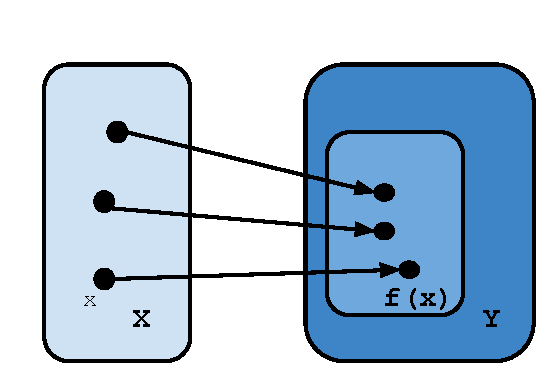
\includegraphics[width=0.5\linewidth]{figs/fn.pdf} 
  \caption{A transformation is only legal if
  the transformed input $x$ is in the set of valid inputs for the API function
  $f$, and the new outcome $y$ is in the set 
  of valid outcomes for $f$. For the network API, this means 
  that the outcome $y$ could have been observed 
  for $f(x)$ on a correct network.}
  \label{fig-fn}
\end{figure}

API calls can be invoked in an 
Affix component by an application or by another component.
The call may then be transformed and invoked in another component, 
or in the network stack of the host \ac{OS}.
Return values from API calls are transformed and propagated to the 
caller in the reverse direction.



\begin{figure}[htb]
  \centering
  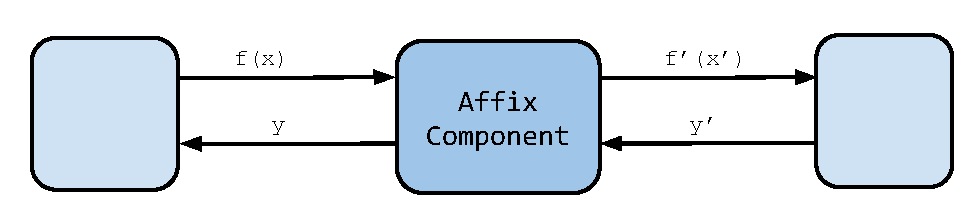
\includegraphics[width=\linewidth]{figs/component_wide.pdf} 
  \caption{An Affix component transforms a function and its input and invokes 
  another component, while returning transformed output
  to its caller. 
  }
  \label{fig-component}
\end{figure}



% Fraidy: I prefer to defer this to the implementation section
%
% The position of Affix components between the application and 
% the operating system's network stack 
% demands that they be compatible with 
% the socket API interface. This is true for both 
% the upwards (presenting a socket interface to the application or 
% Affix component above) 
% and the downwards direction (interfacing with the socket or 
% socket-like structure below it). 
% The Affix component is free in its design of internal workings as 
% long as it respects interface compatibility.

% In practice, interface compatibility requires that an Affix 
% component implements interfaces that match the different 
% groups of operations available on an actual socket, i.e. 
% address resolution (\texttt{getaddrinfo()}), 
% connection management (\texttt{listen()}, \texttt{connect()}, 
% \texttt{accept()}, etc.), 
% data flow (\texttt{send()}, \texttt{recv()} ...), 
% and possibly configuration (in the form of socket options).

% In addition to the interfaces required per the socket \ac{API}, 
% an Affix component must implement a number of Affix-specific 
% functions for instantiation and configuration, including 
% ones for combining multiple Affixes. We will discuss these 
% in an instant.


\subsubsection{Special components}
\label{special}

A particular API call is called \textit{transparent} for a component
if it  preserves interface semantics itself, without
requiring the application of another 
operation. That is, if the component transforms 
$y = f(x)$ into $y' = f'(x')$, and
$y'$ is also a valid output of $f(x)$, then $f(x)$
is transparent in this component. If every API call 
in a component has this property, then the entire component 
is transparent. For example, a \textit{RateLimit} service 
that performs traffic shaping
can be implemented in a transparent component.

In the socket API, the \texttt{send()}
 and \texttt{connect()} calls propagate data and associations, 
 respectively, while the \texttt{recv()} and \texttt{accept()}
 calls consume these.
If a propagating API function $f$ is not transparent for a component, 
then the component must also implement the consuming equivalent function 
$g$ such that the application of $f$ followed by $g$ 
preserves interface compatibility -- i.e., that it gives a 
result that could be observed on a correct network. 
\cappos{Assuming that a component must `mirror' itself... (see later comment
in 5.2)}
For example, if the \texttt{send()} call of a 
\textit{Compression} component 
compresses data before sending it over the network, 
the \texttt{recv()} call of the component should decompress 
received data before returning it to the application.


A component that transforms a propagating 
call into its consuming equivalent, and vice versa,
is called a \textit{mirroring} component. 
Mirroring components also reverse the direction 
of invocation on their output.
The network itself is modeled as a mirroring component, 
as it transforms API calls like \texttt{send()}  
into \texttt{recv()} calls. Figure~\ref{fig-mirroring}
shows how the network transforms a \texttt{send()}
call invoked on one side into a 
\texttt{recv} call on its other side.

\begin{figure}[htb]
  \centering
  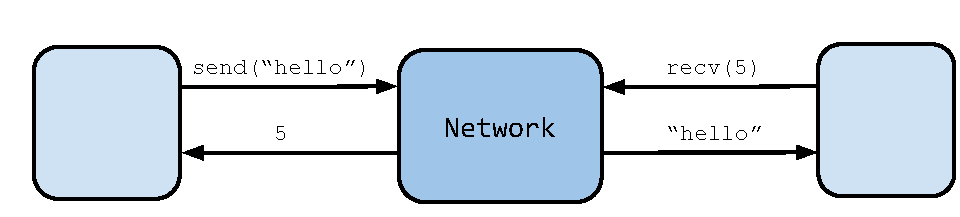
\includegraphics[width=\linewidth]{figs/network.pdf} 
  \caption{The network itself is modeled as a
  \textit{mirroring} component. It transforms calls 
  that propagate (e.g., \texttt{send()}) into 
  calls that consume (e.g., \texttt{recv()}) and 
  reverses the direction of invocation on its output. }
  \label{fig-mirroring}
\end{figure}


Other special components include \textit{manager}
components, which add or remove other components 
and links between components, and
\textit{branching} components, which may invoke 
a function in more than one next component.  
The \textit{Coordination} service discussed 
in detail in Section~\ref{subsec-services-coordination} is a manager, 
and a branching component is illustrated 
in Figure~\ref{fig-tree} (node $A$).


\subsection{Combining Affix components}
\label{subsec-arch-stack}

% \begin{figure}[htb!]
%   \centering
%   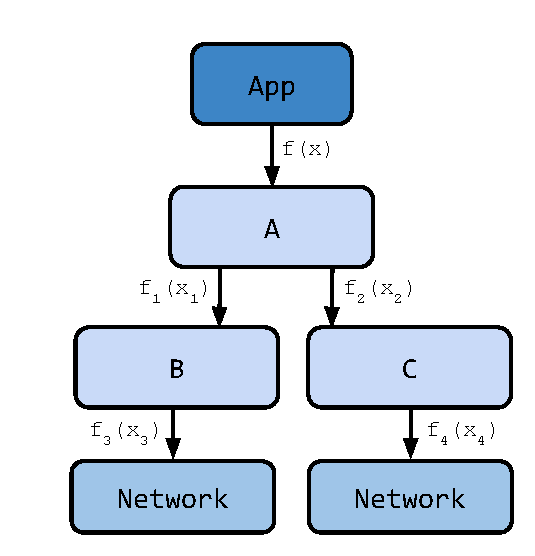
\includegraphics[width=0.7\linewidth]{figs/tree.pdf} 
%   \caption{The set of Affix components operating on one
%   socket form a rooted tree, with arcs showing the 
%   invocation relationship between components.}
%   \label{fig-tree}
% \end{figure}


% Validity of permutations doesn't mean every permutation is meaningful.
Affix components that act on a single socket
in an application
are organized as a rooted tree.
Every Affix component is represented as a 
node in the tree, with arcs showing that 
the source node may invoke calls in the destination node.
A sample tree is given
in Figure~\ref{fig-tree}.

When the application calls an 
API function, the call is handled first by the root node.
Each node in the tree may transform the call
and then one or more child nodes. A
terminal node calls the underlying network API, propagating 
the function call to the \ac{OS} network stack, which in turn 
passes data through the network. 


% Given interface compatibility towards both the next-higher and 
% lower layers means that an Affix component need not necessarily 
% call into the actual \ac{OS} socket, or be called by the 
% actual application from above. Rather, Affix components can be 
% situated on top of one another, a setup we refer to as an 
% \textit{Affix stack}. Through stacking, complex functionality 
% can be assembled from multiple simple Affix components, an approach 
% that follows good design practice -- it advertises reuse, and keeps 
% single Affix components light-weight.

% We required before that the composition of services in a 
% componentized networking framework must be dynamically modifiable 
% for it to achieve maximum impact. Each Affix component is therefore 
% aware that it might live in an Affix stack, and includes functionality 
% to modify the stack below it. Specifically, an Affix component can 
% add or remove other Affix components below it to adapt the stack's 
% capabilities to that of the remote side.



\subsection{Propagation of API calls}
\label{subsec-arch-flow}

When connected through the network (which, 
as described in Section~\ref{subsec-arch-stack}, is itself
modeled as a component), 
the Affix components through which data 
for a particular communication travels make up 
a graph. This graph includes the Affix 
tree at each endpoint, as well as those on relays 
or other middleboxes. 
Figure~\ref{fig-dataflow} shows an example of an Affix graph.

\begin{figure*}[htb]

  \centering
    \begin{tabular}{c c}  
    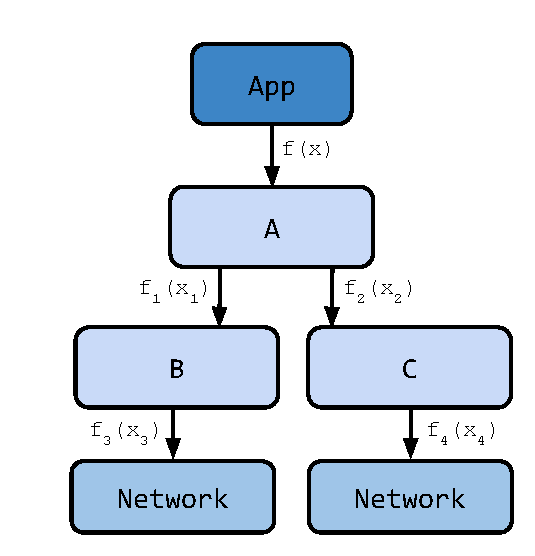
\includegraphics[width=0.35\linewidth]{figs/tree.pdf}  \hspace{.05cm} &
  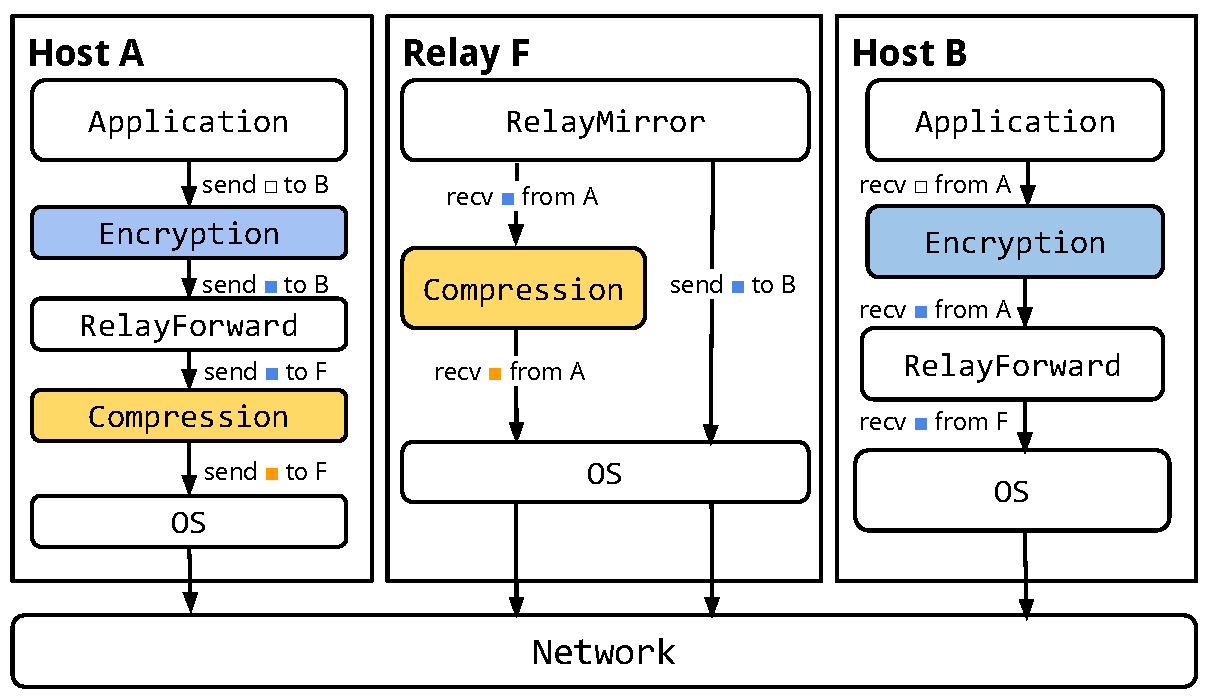
\includegraphics[width=0.6\linewidth]{figs/propagation.pdf}    \\
  \end{tabular}
  \caption{(left) The set of Affix components operating on one
socket form a rooted tree, with arcs showing the 
invocation relationship between components.}
\label{fig-tree}
\caption{(right) This figure shows how Affix components 
  intercept an API call, transform the data and endpoints 
  associated with the call, and propagate the call through 
  an Affix graph until it reaches its destination.}
\label{fig-dataflow}

\end{figure*}

%      \caption{This figure shows how Affix components 
%  intercept an API call, transform the data and endpoints 
%  associated with the call, and propagate the call through 
%  an Affix graph until it reaches its destination.}
%  \label{fig-dataflow}


%  \caption{This figure shows how Affix components 
%  intercept an API call, transform the data and endpoints 
%  associated with the call, and propagate the call through 
%  an Affix graph until it reaches its destination.}
%  \label{fig-tree}



In Figure~\ref{fig-dataflow}, an application on Host A
calls \texttt{send()} with some data to send and a destination
endpoint. This figure illustrates the requirements for 
a path through the Affix graph to satisfy
end-to-end interface compatibility:

\begin{itemize}
 \item Any non-transparent call must be followed by its mirror
 call.
 \item If a function $f$ that is not data transparent is called 
 before a function $f'$ that is also not data transparent, then 
 their mirror functions must occur in the reverse order: 
 $g'$ before $g$. 
\cappos{Stray thought: What if the order is fgf?   (I know the answer
and the reader will too, but we may get this comment from a reviewer.)}
\item Calls that transform the endpoint associated with a call
must be transparent end-to-end, i.e., their composition must 
satisfy the requirements for transparency described in 
Section~\ref{special}.
\end{itemize}


\subsection{Coordination Service}
\label{subsec-services-coordination}
\cappos{Make this more formal.   Leverage the formalisms to define
a calculus for communication in this domain...}

Most Affix services operate on network traffic to improve performance, 
but unlike standard library or other implementations 
of these services, they can be deployed in a democratic fashion. 
However, they do not themselves contribute to democratic deployment. 
In contrast, the function of the \emph{Coordination} service is to 
enable democratic deployment. 

The Coordination service identifies the Affix components used 
by an opposite side of a communication flow, then loads a matching 
set of Affix components on the local host.
This enables communication through any composition
of services without prior arrangement.
The Coordination service described in this section is 
the exemplar service included in the Affix implementation and 
deployed on the Seattle testbed; 
it is also possible to implement alternative coordination services
with equivalent functionality but different properties.


\iffalse

While some Affix components can be used by either side of a 
connection transparently, many components will 
require some level of client-server communication in order 
to work properly. The client and server
needs to balance the Affix stack against each other in order 
to ensure proper communication. Take
for example that the server is using both the CompressionAffix 
and the EncryptionAffix in order
to compress and encrypt it's communication. If a client wants 
to connect and communicate with the
server, than they must also use the proper CompressionAffix 
and EncryptionAffix in order to be able
to decrypt and uncompress the data before returning the data 
to the application layer. In order for
the client to find out that the server is using these two 
components, it needs to be able to communicate
and coordinate with each other to ensure both sides are 
using the same Affix stack.

The practicality of different approachs taken to coordinate 
Affix stack information between clients and servers 
will depend on several factors. Consider the following 
two approaches.  

Approach One: A special purpose Affix component is put in place at the bottom of the network stack. 
Whenever a packet is received this componen willt facillitate communications to ensure the correct 
Affix stack is put into place on both sides of the connection.

Approach Two: A sever decides what Affixes will be used, and advertises the result under an applicaiton 
specific identifier, and port number in a secure look up service.  When a client program wants to connect 
to a server a look up is performed to find out what Affixes should be put into place. 

The first approach had the bennifit of not requireing an outside service, or the overhead added 
by advertisements and look ups.  As long as connection establishement is not an issue coordination 
of Affix stacks in this manner is perferable.  The second approach is, however, the only viable one 
in many situations. Consider for instance that no direct connection can be established to a particular server.  
The server can impose a NatPunchAffix that accepts traffic through a publicly reachable forwarder, 
but the client must some how learn what Affix stack to use in order to connect.  
\fi


The Coordination service implemented in Affix is always placed at the root
of an Affix tree. It redefines \texttt{listen()} to call
\texttt{get\_advertisement\_string()}. This returns a serialized description 
(called an \emph{Affix string})
of all non-transparent services underneath itself in the Affix tree.
The address at which it would like to be reached and the Affix string
with which it can communicate are sent as a key-value pair to 
a public \emph{advertise service}. Finally, the service invokes \texttt{listen()}
in the Affix component beneath itself.

When the opposite host calls \texttt{connect()}, the Coordination service 
queries the advertise service to find the Affix string stored for the 
given destination address. It then constructs a matching Affix tree beneath itself.

\albert{Fraidy noted: ``What is interesting? notable? about this coordination service?''}

\cappos{I was thinking something similar.   I was also thinking another
way to spin this is as protocol / service negotiation...}


\iffalse
Thus we implemented the second approach by leveraging an advertise service in order to
build the CoordinationAffix component which allows the client to do a lookup and build the
Affix stack the server is using, even if the server is directly unreachable. The advertise
service we use consists of multiple servers that are available on public domains. The service
has a redundancy system in order to ensure the service is always available.

The CoordinationAffix on the server side usually lies at the top of the stack and has a view
of all the Affixes that are in the stack. The CoordinationAffix serializes the stack on the
server side and advertises the serialized string on the advertise service. The CoordinationAffix
on the client side does a lookup on the advertise service to retrieve the serialized form of the
Affix stack. The coordination component than deserializes the Affix stack string and builds
the new Affix stack on the client side before making any network calls. Note that the 
CoordinationAffix only serializes the non-transparent Affixes that need to exist on both
sides of communication in order for the two nodes to communicate properly. Examples of such
components are CompressionAffix, EncryptionAffix and NatPunchAffix. The CoordinationAffix
however does not advertise transparent Affixes, such as LoggingAffix, StatAffix and RateLimitAffix.
\fi




\subsection{Naming}
\label{subsec-implementation-discussion}

\cappos{Does this belong earlier?   It ties in well with the deployment
subsection...}

An important aspect of democratic deployability is the ability to support 
communication with legacy (non-Affix) clients and servers.   In other 
words, Affix itself should be democratically deployable.   %To support
%this, there are several important challenges.
%\cappos{We likely need to discuss naming before this...}
However, on the Internet, hosts are commonly identified by 
a DNS name.   The DNS name is then mapped to an IP address.
However neither of these serve as a unique identifier
for a communication endpoint, especially in the presence of NAT boxes.
If we ignore non-Affix applications for the moment, it would be possible
to simply have an Affix endpoint use a Affix ID
as a name in a global registry similar to DNS.   (For scalability reasons,
such a registry can be implemented as a distributed hash table.)
The client could look
up the ID and use the resulting information (such as the serialized 
Affix stack) to understand how to contact the server.   However, this only
will work when both the server and client support Affix.
\cappos{I need your help here.   This text is rough to say the least.}

Applications must work correctly with either a client or a server does not 
support Affix.   If a server does not support Affix but the client does support
Affix, then it is trivial for the client to simply contact the server
without Affix.
However, an unmodified legacy client 
must be able to communicate with an Affix server.   If a legacy client knows
the server's IP or hostname instead of its Affix ID, the client can connect
to the server.
%the client does not know how to connect to a server given an Affix ID.

However, in some cases a server is not directly by IP address (eg when
behind a NAT).
For legacy clients that use a hostname, it is possible to still support
Affix by overloading the existing name.  To do this, a service called 
Zenodotus maps every
Affix ID to a valid DNS name.   A client using a Zenodotus name
(ending in {\tt zenodotus.[anonymized].org}) and it is resolved to an
IP address where the client may contact the server. 
%For example, in Figure~XXX(a), a webserver wants to support compression
%for Affix clients while also supporting legacy clients.   Legacy
%clients will look up the webserver's DNS name and contact it on 1.2.3.4, port
%80.   However, Affix clients will lookup the Affix ID and find that the
%server supports compression on port 8000.   An Affix enabled client can take
%advantage of this support.
%
%Note that the Affix ID for a server need not refer to the host's IP address.
For example, in Figure~XXX, a server behind a NAT is contactable by 
providing the
relay's IP address to legacy clients.   In this example, Affix clients are 
able to connect to the server.   Additionally, clients that support
Affix will benefit from compression and encryption while communicating
over the relay.

%Given a portion of the address space to map names into (such as exists in 
%IPv6), Affix could also support legacy clients that use IP addresses
%instead of hostnames.
%\cappos{Is this too tangental?}



%A legacy client can use the DNS name
%to uniquely refer to the server.  Zenodotus will resolve this to
%an IP address that a legacy client can use to communicate with the server
%(Figure~XXX).   This 
%Affix components that are transparent to the client.
%XXX
%
%However, a server may have different services running on different ports.
%If the same hostname is used, then the same public relay must be used
%for all ports on the server.   This may be less than ideal because different
%applications / flows may want to relay through different systems.   To
%mitigate this, the XXX




\cappos{I'm intentionally dodging ports / protocols because I think it muddies
the water too much.}

\subsection{Deployment paths}
\label{subsec-deployment}
\cappos{Needs to be less implementation specific and more general...}

% Fraidy: I do not like this idea of an "uncooperative"
% application. I also want to focus more on "who" rather 
% than "where"

% There are two orthogonal concerns when deploying Affix with an 
% application: \textit{Cooperation} -- the application might or 
% might not actively expect and liaise with the Affix framework --, 
% and \textit{location} -- Affix components can be deployed at 
% different elements along the network path.

% A cooperative, i.e. Affix-aware, application includes Affix 
% functionality natively by using the  Affix libraries, so that 
% users will benefit without having to explicitly load Affix
% stacks on their own. An uncooperative application can be 
% forced to use Affixes either by relaying its traffic through 
% an Affix-aware \textit{proxy} application (on the same host, or 
% on a separate middlebox), 
% or by \textit{interposition} on its network library calls, 
% e.g. by setting the \texttt{LD\_PRELOAD} variable in Linux so that 
% Affix functions will be used before those of the same name in 
% the standard libraries. 
% Either way, program behavior is modified non-invasively, 
% and it can be configured system-wide 
% or used selectively on a per-application basis.


The Affix framework and core services may be installed as a 
Python package. Once installed, 
there are several methods available for using 
Affix, including:
\begin{itemize}
    \item \emph{Proxy}-based use. The Affix package includes a Python proxy,
which can load an abitrary Affix configuration. 
Traffic must be tunneled through the 
proxy for Affix functionality to be applied.
    \item \emph{Interposition}. The Affix library may interpose on network library calls 
(e.g., by setting the \texttt{LD\_PRELOAD} variable in Linux) so that 
its functions will be used before those of the same name in the standard libraries. 
    \item \emph{Native} integration within an application. A developer can 
choose to include Affix functionality natively in an application using the Python 
library.
\end{itemize}
The first two cases are suitable where the source code of an application 
is not available, where native integration is not practical, and/or when 
Affix is deployed by a non-programming end user.
In both proxy- and interposition-based use, 
program behavior is modified non-invasively, and it can be configured system-wide 
or used selectively on a per-application or per-socket basis.
\cappos{I thought ``How?'' when reading here.   Maybe describe a decider 
component in a sentence.}


% Albert: How about \multirow's and sub-figures?
\begin{figure*}[t]
  \centering
  \begin{tabular}{c c c c}  
  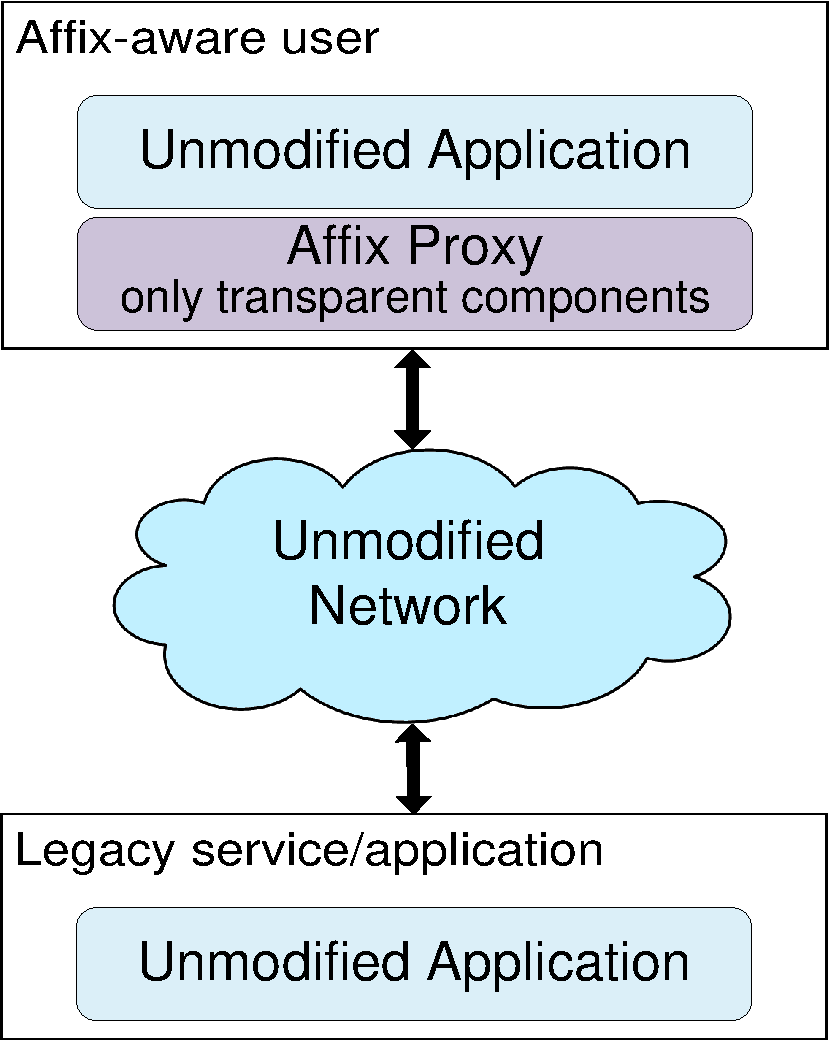
\includegraphics[height=4.75cm]{figs/dep3.pdf} \hspace{.05cm} &
  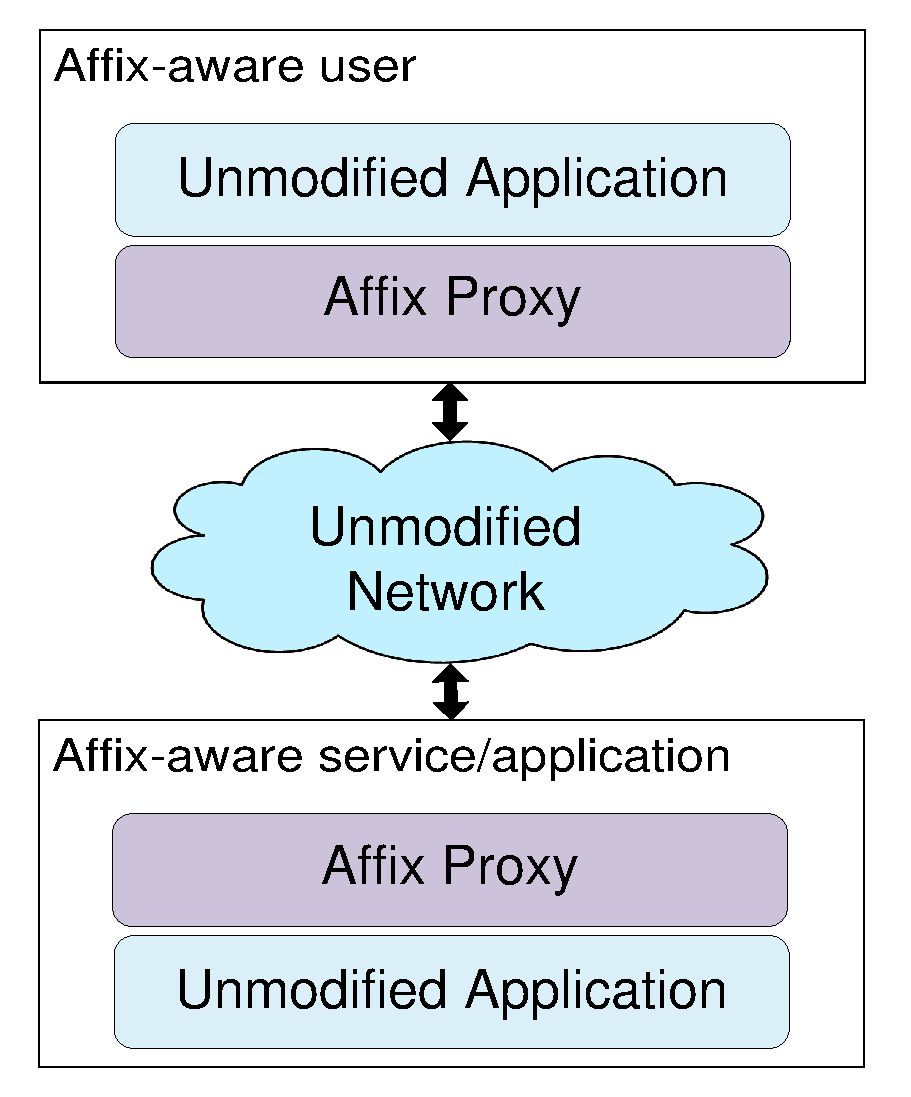
\includegraphics[height=4.75cm]{figs/dep2.pdf} \hspace{.05cm} &
  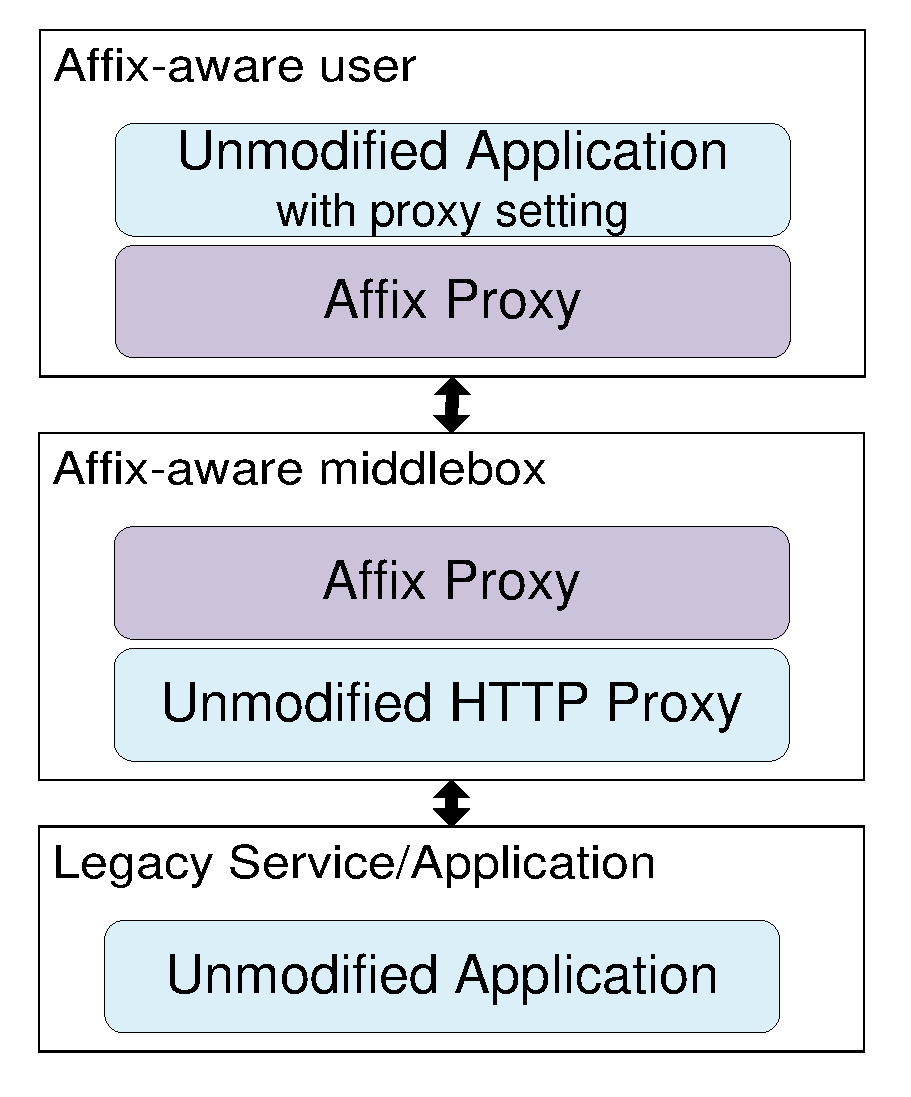
\includegraphics[height=4.75cm]{figs/dep1.pdf} \hspace{.05cm} &
  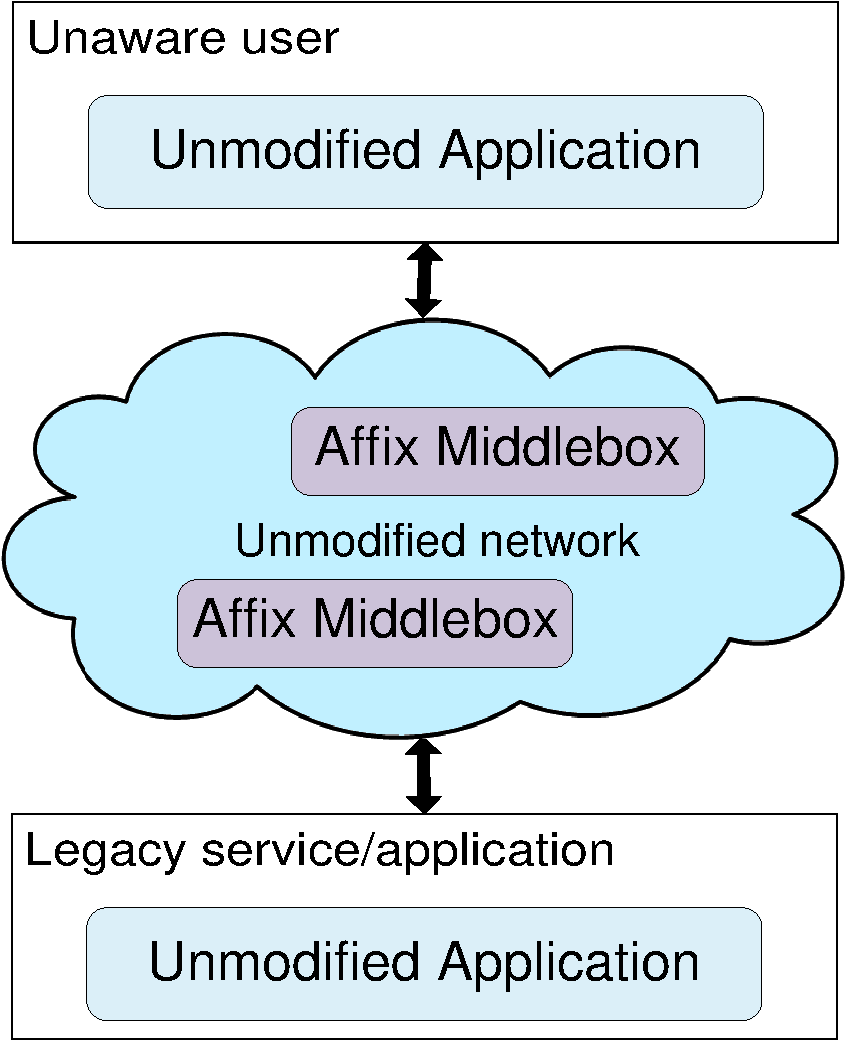
\includegraphics[height=4.75cm]{figs/dep4.pdf} \\
  (a) Only user is  \hspace{.05cm} & (b) User and service \hspace{.05cm} &  (c) User and middlebox \hspace{.05cm} &  (d) Only the core network \\
  Affix-aware  \hspace{.05cm} & are Affix-aware \hspace{.05cm} &  are Affix-aware \hspace{.05cm} &  is Affix-aware
\end{tabular}
  \caption{Affix supports various deployment paths for unmodified applications, depending on which parties are involved. Note that it is possible to use Affix if only the end user is 
  Affix-aware, as shown in Figure~\ref{affix-deployment}(a), 
  as well as when neither end user nor web service provider are Affix-aware, 
  as in Figure~\ref{affix-deployment}(d).   Applications co-located with
an Affix proxy may alternatively be changed to natively support Affix.}
  \label{affix-deployment}
\end{figure*}


Figure~\ref{affix-deployment} shows four possible deployment 
options available for use with unmodified applications
(i.e., the application developer is not a cooperating party). 
These deployment options are especially 
important in the context of democratic deployment, 
and several are unique to the Affix framework:

\begin{itemize}
    \item A user can run an Affix proxy to use transparent 
Affix components (such as rate limiting), and tunnel traffic from applications 
through the proxy, as in Figure~\ref{affix-deployment}(a),
    \item Users on two sides of a connection can run the 
proxy with double-sided Affix components (such as compression or encryption),
and tunnel traffic from applications through the proxy, as in Figure~\ref{affix-deployment}(b),
    \item A user can run the included Affix proxy to use double-sided and single-sided
Affix components, and direct traffic from applications to a proxy elsewhere on 
the Internet that offers Affix functionality, as in Figure~\ref{affix-deployment}(c)
    \item Traffic can be routed through an Affix stack without deploying 
    Affix on any end devices, by applying the interposition 
method on middlebox devices as in Figure~\ref{affix-deployment}(d).
%    \item An operating system can use the interposition method to 
%support Affix functionality with every application,
%    \item An application developer can use Affix components directly 
%within an application,
%    \item An advanced user or application developer can use Affix components 
%directly in a wrapper around an application.
\end{itemize}


%!TEX root = paper.tex
\section{Implementation}
\label{sec-implementation}

%Implementation: 
%  why it's written in repy (especially, how repy helps encourage interface compatibility) 
%  The API including the required calls that a component must implement
%  How a component can manipulate those beneath itself
%  How one uses Affix (native in Python/proxy)
%  Deployment paths (see figure)

In this section, we describe the implementation 
of the Affix platform, a componentized networking 
framework which embodies the goals 
described in Section~\ref{sec-goals}.
Affix allows researchers and developers to create components
that implement networking services, and distribute them to 
end users so that they may be deployed in a democratic fashion.
We describe the design considerations involved in the 
implementation of the platform (Section~\ref{subsec-design}), the general 
structure of the Affix implementation (Section~\ref{subsec-affix}), 
the democratic deployment paths available 
with this implementation (Section~\ref{subsec-deployment}), 
and selected issues that had to be addressed for Affix to work 
unmodified on the current Internet (Section~\ref{subsec-implementation-discussion})

\subsection{Design considerations}
\label{subsec-design}

Several tradeoffs were involved in the design 
of the Affix implementation. In this section, 
we discuss the considerations 
underlying our choice of network API and
level of operation.
 
\subsubsection{Network API}

Affix supports interface compatibility with respect to 
the Repy V2 networking API~\cite{RepyV2API}.
Repy V2 is a language developed for the Seattle testbed
that is conceptually similar to the 
Berkeley socket API. The legacy socket API, however,
is ambiguous in certain cases, and therefore has 
different semantics on different platforms \cappos{cites here}. 
Repy V2 is designed specifically with interface 
compatibility in mind, so that the semantics 
of each call are identical  
regardless of platform.   

This choice is necessarily restrictive. Since not all 
network API calls are supported on all platforms, 
Repy V2 only includes a subset of calls that can be 
made to behave identically on every major \ac{OS}.
This tradeoff is necessary in order to support 
interface compatibility.
\cappos{This is true assuming you don't want to restrict components to an
OS or require every component author to support the quirks of all OSes.}


%While full interface compatibility on one platform prevents a service 
%from passing invalid output to applications on that platform,
%for a networking service 
%to reach the widest audience possible, it should be fully 
%portable across different operating systems and platforms. 
%This means that certain platform-specific functions, 
%or functions with different semantics on different platforms,
%may not be supported. However, we consider the elimination
%of the effort required to port a service to a new platform or OS 
%to be well worth this cost.~\ffund{I moved this 
%text here because it seems like it'll belong here, once 
%we fill out this section.}

\subsubsection{Implementation at the socket API level}

Some classes of networking 
services are indeed faster, more secure, or more capable when implemented 
at a lower layer of the network stack. 
However, there are certain distinct advantages to 
operating at the level of the socket API.
In particular, we argue that certain properties of 
this layer make it more amenable to rapid deployment
of networking services. In this section, we 
describe these properties in more detail.

\paragraph{Leveraging application intent}
\label{subsubsec-intent}
% by sitting close to application layer, we can take 
% advantage of what the application "knows" about 
% its preferences. 
%End to end argument~\cite{saltzer_endend_1984}
\cappos{This is interesting, but I wonder how related it is.   I feel this
point (especially this paragraph) can be trimmed.}
Services situated at lower layers 
commonly make use of information that is lost
as data rises to the top of the network stack (e.g., 
using wireless link quality for handover decisions, 
or link layer loss statistics for congestion control 
at the transport layer).
A similar approach exists for
services operating at higher layers.
Recently, we have seen abstractions such as 
Intentional Networking~\cite{higgins_intentional_2010}
and Socket Intents~\cite{socketintents_2013} 
which enable networking services to use information 
that is gained by being close to the application.

While these examples extend the socket API to more fully support the 
explicit expression of application intent, other implicit expressions of intent 
may be understood just by intercepting socket API calls before they are passed 
to the operating system. Examples of such expressions include the hostname
used to identify an endpoint and the flags passed to a socket API call.
Furthermore, when operating directly at the interface between the application
and the network stack, we can also influence how the application perceives
the network by tailoring the socket API error codes that are raised to the 
application. 
\cappos{You want to make it clear that this is useful for supporting apps
without modification.   That tie in is clear to me but may be missed by
some readers.}

\paragraph{Fine-grained application}
Networking services at lower layers generally require 
either static configuration policies
or reactive adaptability to network conditions
to determine whether a service is engaged for a given 
communication flow. By operating at the socket API layer, 
we gain the ability to apply functionality 
on a per-socket basis.


\paragraph{Operation in userspace}
Because it runs above the 
operating system's network stack, a socket API-level service 
can be implemented completely in userspace. Although
userspace services can incur a performance penalty, 
they may also be installed and operated without superuser 
privileges in many cases. As processing power becomes 
increasingly inexpensive, the performance gains associated 
with operating in the kernel or in hardware become 
less necessary and the relative benefit of allowing deployment 
by unprivileged users becomes more significant.


\iffalse
\paragraph{Support for legacy applications, hosts, and networks}
To encourage deployment, a service should not require
changes to the code base of an application, the operating system 
of an end host, or the devices and links that make up a network.
By operating outside of these entities, a socket API-level service 
loses the opportunity to leverage application-specific 
or network-specific context (except for the kind 
of context described in Section~\ref{subsubsec-intent}).
However, this enables it to support oblivious applications, 
hosts, and networks, as required for democratic deployment.
\fi

\subsection{Implementing an Affix Component}
\label{subsec-affix}

The Affix software release includes the Affix framework -- the infrastructure 
necessary to construct and send traffic through an Affix tree -- 
as well as a set of core components.

Affix components implement new functionality as follows.
Each Affix component overloads the network API calls in the 
Repy V2 API, which includes all the functions necessary to initiate, 
connect, and send and receive data through a TCP or UDP socket.
The logic for a new network service is implemented inside
these overloaded functions.
A component that does not tranform a particular call simply 
invokes the same function 
with the same arguments in its child.


Each component is also required to define a \texttt{copy()}
call and a  \texttt{get\_advertisement\_string()} call.
These functions are necessary for managing and 
coordinating the Affix graph..
The \texttt{copy()} function makes a complete 
copy of the component itself, 
including any relevant configuration options.
The \texttt{get\_advertisement\_string()} must give 
all the information necessary to mirror the component.
For a transparent component, this function usually 
returns an empty string; for non-transparent components
it typically 
\cappos{This seems to imply components do not always mirror themselves.}
describes its own name and configuration.


The Affix framework itself includes functions to construct a tree,
observe a subtree, add or remove arcs from the tree. 
The direction in which these functions may be invoked is the 
same as the direction in which network API functions are 
invoked. Thus, a component may construct 
a new subtree and add an arc from itself to that tree;
but it may not, e.g., remove the link between itself and its parent.
These functions enable the construction of an Affix graph 
at connection time (i.e., the property of dynamicity), 
so that interoperability can be ensured without prior agreement
 between endpoints.


 \iffalse


Affix components are built on top of the Repy API and thus must implement
all the network API calls~\cite{RepyV2API} from Repy that are semantically consistent with
the API. The framework provides an Affix component called \textit{BaseAffix}
which defines all of these API calls along with some extra internal API calls.
Every Affix component that is built, should inherit the BaseAffix class 
and may overload any of these network API calls. 

In addition to the network API calls, each Affix component must overload the
two API calls: copy() and get\_advertisement\_string(). The function
copy() must make a copy of the Affix component itself, copying over any values
and variables that is relevant to the Affix component. The call get\_advertisement\_string()
returns a representation of the Affix component as the component wants to be seen. The Affix
component may include any data in this advertisement string as it wishes to. Most 
transparent Affix components such as LogAffix or StatAffix will return an empty string.
This advertisement string is used mainly by the CoordinationAffix to balance 
the Affix stack on both sides of the communication. More details on the CoordinationAffix
is provided in Section~\ref{subsec-services-coordination}.

Each Affix component also has functionalities that allow it to modify the Affix
stack underneath it. In the next section we describe some of these functionalities
and how they can be used to manipulate the Affix stack.

In the simplest case, a Noop Affix would have to inherit the BaseAffix and would
need to only overload the functions copy() and get\_advertisement\_string(). As
the Noop Affix will not be changing any of the network calls, it will not be 
required to overload any of the network API calls.


\subsection{Affix Stack Manipulation}
\label{subsec-affixstack-manipulation}

In Section~\ref{sec-architecture} we introducted the concept of \textit{Affix stack},
which is a composition of multiple Affix components on top of one another. The 
purpose of an Affix stack is to allow the user to address multiple networking 
challenges simultaneously by stacking multiple Affix components. Various Affix stack
APIs are provided to allow users to view and change the Affix stack that they have
built. These functionalies allow users to view every Affix component that is in the
stack as well as add, remove or change the order of the Affix components in the
stack. The list of API along with their description can be found in 
Table~\ref{tab-affixstackapi}. The calls \texttt{push()} and \texttt{pop()} can 
be used to modify the Affix stack during any network calls. It should be noted 
that individual Affix components have the ability to modify the stack underneath
them, however they cannot modify the portion of the stack above them.

There are many situations where one side of the network connection might want to 
modify the stack without the other side modifying their side. An example of such
a scenario is when one side of the network connection wants to use transparent 
Affix components. The user may want to monitor all network communications with
Affix components such as LogAffix or StatAffix in order to keep track of all 
the network calls made as well as statictics on the data flow. Users may also
want to use one sided Affixes such as DataLimitAffix or RateLimitAffix in order
to control the amount of data that is uploaded/downloaded by the application or
to control the throughput of the application.

Applications may also be using \textit{Decider Affixes} that enforce the Dynamicity
property that is desired by the Affix framework. Examples of such an Affix component
would be the NatDeciderAffix, which evaluates the network connectivity and determines
whether the node is behind a NAT or not. If the node is behind a NAT, the NatDeciderAffix
would modify the Affix stack by adding in the NatPunchAffix underneath it in order
to allow the node to perform NAT traversal in order to receive incoming connection.
Another example of a Decider Affix would be a simple UDPFecDecider Affix that monitors
the data loss and may decide to load the FECAfffix in order to reduce data loss if 
the connectivity has a high data loss rate.

\subsection{Properties of an Affix Stack}

In order for an Affix stack to function properly, it needs to meet certain properties.
Below we discuss several of it's properties and how a stack may behave under certain
scenarios.

\subsubsection{Semantics of Individual Affix Components}

Each individual Affix component that resides in the Affix stack must be semantically
consistent with the networking API, in this case with Repy. If any of the components
are not consistent with the network API, than an unwanted exception or undesired behaviour
may be raised by the Affix stack to the application layer. This is highly undesirable
as this will break the \textit{Interface Compatibility} property of the Affix framework.
Furthermore, if a component breaks semantics, it may not be permutable with other Affix
components, breaking the \textit{Permutability} property. 

\subsubsection{Building the Affix Stack}

Our implementation builds the Affix stack when the stack is 
initialized by the user rather than building the stack right before the network
call. Building the stack at initialization allows the Affix framework to verify
that each individual Affix components can be loaded properly. This also ensures
that the Affix framework does not raise any internal error during the network call
in case an Affix component cannot be loaded or initialized properly.

\subsubsection{Copying an Affix Stack}

When a network call is invoked, there are cases when the Affix stack is copied
before making the network calls and there are cases when a new Affix stack is
created instead of a copy being made. There are two simple situations between
when a stack is copied versus when a new stack is created. 

The original Affix stack is used when network calls create only one new socket. 
For example, the API calls: listenforconnection(), listenformessage(), openconnection() 
and sendmessage() should use the original Affix stack. The reason being, these calls 
are invoked once and creates one individual sockets that will be used for the rest 
of the communication. For example, every time the calls openconnection() and sendmessage() 
is invoked, a new socket is created that can be used for the rest of communication. 
Similarly when TCPServerSocket.listenforconnection() and UDPServerSocket.listenformessage() 
are invoked, a new listening
socket is created that will be used for accepting any new incoming connection.

A copy of the Affix stack is made for network calls that create new sockets that 
inherit the property of the parent socket. For example, the network calls getmessage() 
and getconnection() should create a copy of the Affix stack before using the stack. 
A copy of the stack is created first when the calls getmessage() and getconnection() 
are invoked because these calls  may be called multiple times and each call will create 
a new socket-like object which inherits the properties of the parent socket. These 
socket-like objects will inherit the Affix stack of the parent socket and each individual 
socket has the ability to modify the Affix stack that they inherited, independent of it's
parent or sibling sockets.

The EncryptionAffix is a good example that displays the necessity of copying the Affix
stack in certain cases. If the EncryptionAffix is being used, the EncryptionAffix 
generates a new set of key for use between the two endpoints of communication. If 
the same Affix stack is used by the sockets created when invoking the calls 
UDPServerSocket.getmessage() and TCPServerSocket.getconnection(), than all the 
children sockets would be forced to use the same key for communication. Thus a 
copy of the stack needs to be made in order for the child sockets to use different
keys for encryption. On the client side however, when the calls sendmessage() and 
openconnection() are invoked, a new socket is created that does not inherit from
any parent socket. Thus the original Affix stack may be used for communication as
each socket created by these calls have different instances of the Encryption Affix
component.
\mmm{Feel free to rewrite this section, if the wording is off.}

In the next section we describe the various Affix components that we have built as
sample components for the Affix framework.
 

\begin{table}[t]
\scriptsize
\centering
\begin{tabular*}{\columnwidth}{|l|p{4.95cm}|}
\hline
Affix Stack API & Description \\ \hline
\hline
peek() & Returns reference to the next Affix component in the stack that is right below the current Affix component. Raises an error if current stack is empty.  \\ \hline
pop() & Will remove and return the Affix component that is right below the
current Affix component. Raises error if the current stack is empty.  \\ \hline
push(affix\_component) & Pushes the specified Affix component below the current
Affix component. If we are at the top of the stack, the component is pushed to 
the top. \\ \hline
\end{tabular*}
\caption{List of Affix stack API.}
\label{tab-affixstackapi} 
\end{table}
\fi

\iffalse


The AFFIX framework is implemented in the subset of Python supported by version 2 
of the Repy API developed for the Seattle testbed.  The networking portion 
of this API is conceptually similar to the 
Berkeley socket API. Unlike the legacy socket API, however, Repy API operations 
are defined unambiguously and are semantically identical on all 
supported platforms~\cite{RepyV2API}.
\ffund{What does this mean? elaborate.}   

To encapsulate functionality in an AFFIX component, a programmer needs only 
to override the existing Repy API functions with new functionality. 
In addition to standard networking functions such as \texttt{send}, \texttt{listen},
and \texttt{recv}, an AFFIX component may also include functions to 
operate on or describe (by means of an AFFIX string) the AFFIX tree beneath itself.



\begin{table}[t]
\scriptsize
\centering
\begin{tabular*}{\columnwidth}{|c|l|p{3.05cm}|l|} 
\hline
~ & Shim& Description& LOC \\ \hline
\hline
\rownumber & RSA & - & 217 \\ \hline
\rownumber & NatPunch & - & 172 \\ \hline
\rownumber & Compression & - & 208 \\ \hline
\rownumber & HideSize & - & 183 \\ \hline
\rownumber & FEC & - & 127 \\ \hline
\rownumber & AsciiShifting & - & 16 \\ \hline
\rownumber & RateLimit & - & 112 \\ \hline
\rownumber & OneHopDetour & - & 98 \\ \hline
\rownumber & DataLimit & - & 78 \\ \hline
\rownumber & UdpOverTcp & - & 171 \\ \hline
\hline
\rownumber & CoopShim & - & 202 \\ \hline
\hline
\rownumber & Log & - & 162 \\ \hline
\rownumber & UdpLoss & - & 41 \\ \hline
\rownumber & NoopShim & - & 5 \\ \hline
\rownumber & CheckAPI & - & 725 \\ \hline
\hline
\rownumber & Coordination & - & 136 \\ \hline
\rownumber & MultiPath & - & 280 \\ \hline
\rownumber & UdpMultiPipe & - & 138 \\ \hline
\rownumber & UdpCompressionDecider & - & 49 \\ \hline
\rownumber & UdpFECDecider & - & 41 \\ \hline
\rownumber & BindLocalAddress & - & 34 \\ \hline
\rownumber & Mobility & -  & 281 \\ \hline

%CheckAPI & Validates network API semantics & 725 \\ \hline
%Coordination & Builds a balanced shim stack & 128 \\ \hline
%Compression & Compresses data  & 201 \\ \hline
%DataLimit & Restricts volume of traffic over a period & 78 \\ \hline
%RateLimit & Restricts bandwidth utilized & 112 \\ \hline
%ForwardErrorCorrection & Writes error recovery UDP datagrams & 129
%\\ \hline
%Logall & Logs all network calls and traffic & 162 \\ \hline
%%X logflows & Logs network flow information & XXX \\ \hline
%Duplicate-UDP & Sends data over multiple shimstacks & 139 \\ \hline
%Spiltter-TCP & Splits data, favors fast shimstacks & 274 \\ \hline
%%X branch & Accepts connections from multiple shimstacks & XXX \\ \hline
%NAT-TURN & TURN-like protocol for NAT traversal & 139 \\ \hline
%X NAT-decider & Adds the next shim if one is behind a NAT & XXX \\ \hline
%X reverse-connection & Reconnects from server to client & XXX \\ \hline
%mobility & Handles IP address changes & XXX \\ \hline
%One-Hop-Detour & Routes traffic through a relay & 98 \\ \hline
%Encrypt-rsa & Encrypts traffic using RSA & 206 \\ \hline
%Encrypt-rot & Encrypts with a Caesarean cipher & 16 \\ \hline
%noop & Does nothing & 5 \\ \hline
\end{tabular*}
\caption{Currently implemented shims.}
\label{tab-implementedshims} 
\end{table}

To confirm the utility of encapsulating network functionality in the socket API, 
we created some sample AFFIX components.  Table~\ref{tab-implementedshims} 
lists these components and the LOC count for each.   

\ffund{Write descriptions in table}
Lines 1-10 in Table~\ref{tab-implementedshims} describe shims 
that encapsulate very simple, but highly practical, pieces of networking functionality.
Next the CoopShim component, which implements the hybrid network packet recovery 
scheme described in~\cite{sinkar2008cooperative}, is given as an example of a 
shim that encapsulates more advanced functionality.

The following four lines (12-15) describe some debugging shims that have proved to be useful 
in developing and evaluating AFFIX performance. 

The remainder of Table~\ref{tab-implementedshims} describes ``helper'' components
that act on some way on the AFFIX tree. The first of these is the coordination shim. 
When used as the root node of an AFFIX tree, the coordination 
shim balances AFFIX trees across two ends of a communication flow.
It leverages the Seattle testbed's advertise service, which is conceptually 
a single hash table,  as the
global naming service for the coordination procedure described in~\ref{stack:coordination}.

Among the other ``helper'' components are \emph{decider} shims
that insert or remove nodes beneath itself in the AFFIX tree, \emph{splitter} shims
that stripe traffic across one or more children, \emph{multiplier} shims
that duplicate traffic through one or more children, and a mobility shim that 
enables the AFFIX tree to transparently cross network boundaries.
A complete treatment of these special AFFIX components and particularly their implications 
for dynamic context-aware network use is deferred to a later work. 


\fi


\iffalse
This section describes our implementation of the shim framework.  After describing the overall implementation in Section~\ref{implementation-overview}, we describe how we add shims to unmodified existing applications, summarize some implemented shims, and describe our experiences in designing and building shims.
 
%This includes optimizations to the lookup service to reduce load (Section~\ref{caching})
%authenticity of shim stack data 

%cutting for space

%\begin{table}[t!]
%\scriptsize
%\centering
%\begin{tabular*}{\columnwidth}{|l|l|} 
%\hline
%API Call & Description\\ \hline
%\hline
%
%openconnection & Opens a TCP connection, returns streamsock. \\ \hline
%
%listenforconnection & Listens for TCP connections, \\
%\hfil & returns tcpservsock. \\ \hline
%
%tcpservsock.getconnection & Accepts a TCP connection, \\
%\hfil & returns streamsock. \\ \hline
%
%streamsock.send & Sends data over TCP. \\ \hline
%
%streamsock.recv & Receives data over TCP.\\ \hline
%
%
%sendmessage & Sends a UDP packet. \\ \hline
%
%listenformessage & Listen for UDP datagrams, \\
%\hfil & returns udpservsock. \\ \hline
%
%udpservsock.getmessage & Recieves a UDP datagram. \\ \hline
%
%getmyip & Return the Internet facing IP / hostname. \\ \hline
%
%*.close & Closes a streamsock, tcpservsock, \\
%\hfil & or udpservsock. \\ \hline
%
%\end{tabular*}
%\caption{Seattle network API at a glance.\label{tab-APIcalls}
%JAC: A likely candidate to be cut.}
%\end{table}

\subsection{Implementation Overview}
\label{implementation-overview}

Our work with shims was motivated by our experiences trying to support nodes 
participating in the Seattle testbed~\cite{Seattle_SIGCSE09,Seattlewebpage}.
Any Internet connected device can become a Seattle node by simply running 
the Seattle software.  This software runs along side the users other 
applications and has performance and security isolation.
Seattle runs on end user devices including everything from servers, desktops, 
laptops, tablets, and phones.   Approximately 75\% of the total Seattle users 
are home users.   As such there is a great deal of network diversity including
mobility, nodes behind NATs, low-bandwidth nodes, as well as nodes behind 
organizational firewalls.

Our implementation leverages the Seattle testbed's advertise service as the
global naming service.
% (Section~\ref{sec-coordinate}).   
While Seattle's advertise service is conceptually
a single hash table abstraction, for robustness it uses three separate 
services underneath, the Digital Object Registry~\cite{dor}, Seattle's
centralized advertise service~\cite{centralizedadvertise}, and 
OpenDHT\cite{Rhea_SIGCOMM_2005}.   We constructed a gns-dns mapping
service for legacy applications (Section~\ref{sec-legacy}) called
Zenodotus~\cite{Zenodotus}.

We implemented our prototype in the subset of Python supported by the Repy V2 
API for the Seattle testbed.  This API is conceptually similar to the 
Berkeley socket API, however it is 
semantically defined in an identical manner regardless of the 
platform~\cite{FutureRepyAPI}.   

%The API consists of the calls listed in 
%Table~\ref{tab-APIcalls}.

A shim is an object that has all of the same functions as the Seattle API.
To encapsulate functionality, a programmer simply overrides the functions they
want to change with new functionality.   Besides networking functions, 
there are also functions to copy, serialize, and deserialize shim stacks.   
These routines are used to coordinate a balanced shim stack
and instantiate it.  

Each shim also contains a reference to the shim stack(s) beneath it.   The shim stack 
possesses functions to push, pop, and peek at the next shim in the shim 
stack.   These features are primarily used by decider shims to manipulate
the functionality that is used beneath them.   

\subsection{Deploying Shims}
\label{sec-add-application}

\ffund{This is a good place to mention the benefits of having multiple paths to 
deployment: a tech-savvy 
user may deploy on his own initiative, a developer can integrate into 
application, an OS or device manufacturer could deploy systemwide.}

\ffund{Make sure to explicitly state that every deployment path besides for native 
does ***not*** require modifying the source of an application}

\ffund{ToDo: A ***very simple*** figure illustrating the various deployment methods.}

\ffund{ToDo: include interposition work.}

%In order for shims to be useful, they must be used by an application.
There are several techniques we use to add shims to a program without
modifying them.  For Seattle applications, we leverage the interposition
mechanisms that are inherent in the Repy V2 API.   This interposition 
mechanism, called security layers in other work~\cite{Cappos_CCS_10}, allows
functionality to replace the usual API calls for the sandbox.   As a result,
the usual networking calls are mapped to use shims.   Adding shims in this way
is very lightweight, adding only a few microseconds of delay and around 1KB of 
memory per shim in addition to whatever the shim's functionality requires.

Note that the use of security layers also provides
an inherent security boundary here if desired.   For example, if the owner
of the machine wants to rate limit Seattle applications, they can do so
by including a rate limit shim in a security layer and failing to
map the shim stack object (which precludes access to pop).   

%what is the second  mechanism??  if time permits, we should elaborate...
We also use shims in legacy applications like Apache.   
%We do this by one of two mechanisms.   First, 
We have constructed a legacy relay
program which supports shims (Section~\ref{sec-legacy}).   By running 
a relay on both the client and the server, the traffic is tunneled through
shims.   This obviously does not require any modification to the application.
We have found this simple to run in practice, but does not work for 
applications that perform actions outside of the API.   For instance, an 
application that sends traffic that is not TCP or UDP will not have its 
traffic correctly routed through our relay.   However, most applications do 
not need this functionality and so will work fine using a legacy relay.  Moving forward,
we plan to explore interposing on legacy applications using a 
library or system call interposition mechanism like {\tt LDPRELOAD}.



\subsection{Sample Shims}
\label{sec-examplelayers}

To test the feasibility of encapsulating network functionality in shims, 
we constructed many example shims.   Table~\ref{tab-implementedshims} 
shows a list of the shims and provides the LOC count for each shim.   
Note that about 57 LOC are boilerplate template code that defines the
methods and return values added by each shim.   All of our shims were
implemented by undergraduate students.   

We semantically validated each shim by running it with the checkAPI shim.   
This was very useful in detecting semantic violations and helped us 
debug our shim implementations.   

\eat{
\subsection{Experiences}

%JAC: I don't really know what to do with this, but it seems we need some
%section like this.   Danny has some good information in his thesis we 
%should be able to use.

%Danny: 
Preserving the semantic-consistency comes with a cost: shims
can be difficult to implement.  For example, consider our compression shim.
A compression library that is not concerned with being semantically-consistent
simply breaks up an input stream into distinct chunks, applies compression, and 
sends individual compressed chunks over the network. The Seattle sockets, however, are
non-blocking. Any stage of message segmentation, compression, and
transmission may be interrupted. The compression shim, therefore, has to keep
track of the state of all these stages. It should be able to recover
from an interrupted state if the application decides to resume
transmission at any time. A simple compression library would take less than 100
lines of Python code. Our compression shim consists of 200 lines. It
requires considerable effort to design, implement, and debug. 
}
%(Danny: In my thesis, I also mentioned a number of limitations. Refer
%to the content page. The paragraph above does not appear in the
%thesis.) 

%Throughout the process of implementing shims, we discovered many lessons
%that helped us to think more clearly about network semantics.

%Repeated lookups by the coordination shim can generate a fair amount of
%traffic for the advertise service.   To mitigate this, we cache global
%naming service information for a short period of time (30 seconds).   Much 
%like DNS caching, this prevents repeated lookups at the cost of increasing
%the chance of receiving stale information.



%\subsection{Caching in Lookups}
%\label{caching}

%A potentially significant amount of overhead could come from looking up shim stack information in the advertise service.   Much like in DNS, our solution is to use caching. Assuming that the server's shim stack is not changed over a short period of time, the client's coordination shim caches the contents of the server's shim stack. Any subsequent new connection to the server will read from the cache. 

%In very rare cases, we discovered that obsolete network content was used by the client.   To mitigate any potential impact from this, we modified the coordination shim to detect this problem and flush the cache entry.  

\fi






%\input{services}
%\input{results}
%\input{casestudy}
%\input{conclusion}

%\section*{Acknowledgments}

\footnotesize
%\renewcommand{\baselinestretch}{0}
\bibliography{bibdata}

\end{document}

